\documentclass{report}
\usepackage{amsmath}
\usepackage{siunitx}
\usepackage{eurosym}
\usepackage[utf8]{inputenc}
\usepackage[english]{babel}
\usepackage{array, float}
\usepackage{colortbl}
\usepackage{booktabs}
\usepackage{multirow}
\usepackage{amsfonts, amssymb, amsxtra, amsmath, amsbsy} % Não usar empheq.
\usepackage{adjustbox}
\usepackage{enumitem}
\usepackage{caption}
\usepackage{subcaption}
\usepackage{centernot}
\usepackage{comment}

\usepackage[legalpaper, margin=1in]{geometry}

\usepackage{xcolor}
\usepackage{listings}
\usepackage{ifthen}

\usepackage{graphicx}
\newcommand{\heart}{\ensuremath\heartsuit}

\usepackage{tikz}
\usepackage{pgfplots}
\usepackage{pgfplotstable}
% \usepackage{3dplot}
\usepackage{pgfcalendar}
\pgfplotsset{compat=newest}
\usepgfplotslibrary{groupplots}
\usetikzlibrary{
  arrows,
  positioning,
  matrix,
  calc,
  decorations.pathreplacing,
  decorations.pathmorphing,
  decorations.markings,
  decorations.text,
  shapes,
  backgrounds,
  shadows,
  trees,
  fit,
  snakes,
  patterns,
  mindmap,
  intersections,
  automata,
  plotmarks,
  positioning,
  decorations.pathreplacing,
  spy,
  calligraphy}

\tikzset{every picture/.style={font issue=\footnotesize},
         font issue/.style={execute at begin picture={#1\selectfont}}
        }

\newcommand*\circled[1]{\tikz[baseline=(char.base)]{
            \node[shape=circle,draw,inner sep=2pt] (char) {#1};}}
\DeclareSIUnit{\pers}{pers}
\DeclareSIUnit{\EUR}{\text{\euro}}
\sisetup{
  per-mode = fraction,
  inter-unit-product = \ensuremath{{}\cdot{}},
}

%% biber processes the reference db
%% citation keys and entries will be alphabetic
%% A reference section will be added to each chapter
\title{Macroeconomics and monetary theory}
\author{Nam Pyo Suh}
\date{February 2, 2018}
\begin{document}


\part{First Test Test}
\chapter{How money is created (and destroyed) in modern economies}
\section{Monetary base and money}

$$MB=\text{Notes} + \text{Coins}$$ 2323232 Money is issued by the Central Bank in circulation. So the monetary base is the amount of notes and coins in Circulation plus the the amount notes and coins in Reserves. 

Money, is the means of payment, the titles owned by households, businesses and the state, used for:
\begin{itemize}
    \item buying goods and services; 
    \item pay incomes; 
    \item pay debts.
\end{itemize}

$\text{Titles}=c+CD \longrightarrow $ Notes and coins circulation plus checkable deposits.

\begin{figure}[H]
    \centering
\begin{tikzpicture}[scale=1.5, node distance = 4 em]
\draw node[left]{Money}(0,0) -- (0,2);
\draw(0,2) node[left]{MB} -- node[pos=0.5,sloped,above]{C}(2,2)node[pos=0.5,sloped,below]{1 euro} -- node[pos=0.5,sloped,above]{R}(4,2)node[pos=0.5,sloped,below]{1 euro} -- (6,0);
\draw (0,0) -- node[pos=0.5,sloped,above]{1 euro}(2,0)node[pos=0.5,sloped,below]{C} -- node[pos=0.5,sloped,above]{100 euro}(6,0)node[pos=0.5,sloped,below]{CD};
\draw (2,2) -- (2,0);
\end{tikzpicture}
    \caption{The relation between money balance and money}
    \label{fig:my_label}
\end{figure}

\clearpage
\section{The old view of money creation}

Assumption: $r=\frac{R}{CD}=\frac{10\text{\euro}}{100\text{\euro}}=10\% \implies$ banks have to back their checkable deposits at a fixed ratio.


\begin{figure}[H]
    \centering

    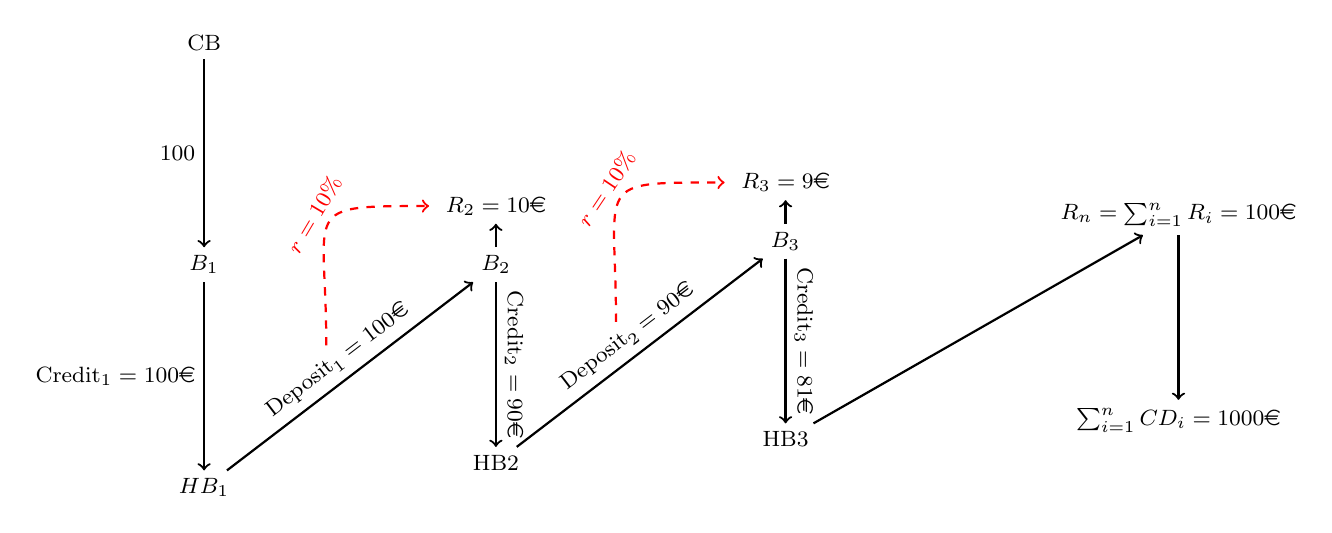
\begin{tikzpicture}[node distance = 8 em and 10 em]
    \node (CB) {CB};
    \node [below = of CB] (B1) {$B_1$};
      \node [below = of B1] (HB1) {$HB_1$};
        
        \node [above right = of HB1](B2){$B_2$};
         \node [above = 1em of B2](R2){$R_2 = 10 \text{\euro}$};
            \node [below = 7em of B2](HB2){HB2};
            
                    \node [above right = of HB2](B3){$B_3$};
                             \node [above = 1em of B3](R3){$R_3 = 9 \text{\euro}$};

                                \node [below = 7em of B3](HB3){HB3};
                                
                                
                                        \node [above right = of HB3](BN){$R_n = \sum^{n}_{i=1} R_i=100\text{\euro}$};
                                                    \node [below = 7em of BN](HBN){$\sum^{n}_{i=1} CD_i=1000\text{\euro}$};






    \draw[thick, ->] (CB) -- node[pos=0.5,sloped,left, rotate = 90]{\footnotesize {$100$}} (B1);
       \draw[thick, ->] (B1) -- node[pos=0.5,sloped,left, rotate = 90]{\footnotesize {$\text{Credit}_1 = 100 \text{\euro}$}} (HB1);
         \draw[thick, ->] (B2) -- (R2);
                  \draw[thick, ->] (HB1) -- node[pos=0.5,sloped,above](D1){$\text{Deposit}_1 = 100 \text{\euro}$} (B2);

                  \draw[thick, ->] (B2) -- node[pos=0.5,sloped,above]{\footnotesize {$\text{Credit}_2 = 90 \text{\euro}$}}(HB2);
                           \draw[thick, ->] (HB2) -- node[pos=0.5,sloped,above](D2){$\text{Deposit}_2 = 90 \text{\euro}$} (B3);
                                    \draw[thick, ->] (B3) -- (R3);


                                    \draw[thick, ->] (B3) -- node[pos=0.5,sloped,above]{\footnotesize {$\text{Credit}_3 = 81 \text{\euro}$}} (HB3);
                                    
                                                      \draw[thick, ->] (HB3) -- (BN);
                                                                                                            \draw[thick, ->] (BN) -- (HBN);



\draw[red, dashed, thick,->,shorten >=3pt] (D1.north) to [out=90,in=180,loop,looseness=2] node[pos=0.5,above, sloped]{$r = 10 \% $} ( R2.west);
\draw[red, dashed, thick,->,shorten >=3pt] (D2.north) to [out=90,in=180,loop,looseness=2] node[pos=0.5,above, sloped]{$r = 10 \% $} ( R3.west);





    \end{tikzpicture} 

        \caption{Caption}
\end{figure}

%scheme of the old view of monetary creation%

\begin{equation*}
    \begin{aligned}
        \sum^{n}_{i=1} R_i=100\text{\euro} \\
        \sum^{n}_{i=1} CD_i=1000\text{\euro}
    \end{aligned}
\end{equation*}

Lesson: 
\begin{itemize}
    \item Money (CD) is created by the initiative of the CB to create reserves. 
    \item The quantity of money in circulation is fixed and determined by the quantity of MB, created by the CB. 
    \item Money is exogenous to the economy. 
\end{itemize}

\section{The new view of Money Creation (BOE, 2014)}

\begin{enumerate}
    \item The CB does not fix the quantity of reserves injected in the banking sector. It sets the interest rate at which it lends reserves to banks. Say $i_{CB}=1\%$. 
    \item Banks add a margin (spread) and set an interest rate, $i$, at which they lend to HBS. Say $i_{C}=3\%$.
    \item At rate $i$, HBS ask for a certain amount of credit, say 150\euro. 
    \item No matter whether banks own reserves or not, they grant the amount they deem credit worthy, say 100\euro ($=\frac{2}{3}$).
    \item They do this not by providing notes and coins, but by opening a checkable deposit (CD) of 100\euro.
\end{enumerate}

\begin{figure}[H]
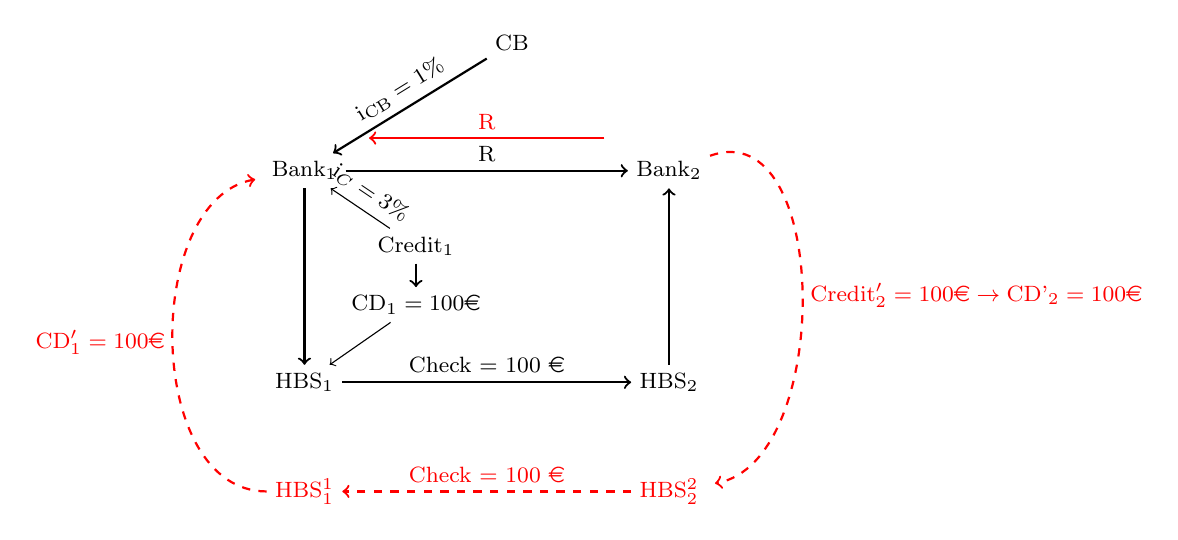
\begin{tikzpicture}[node distance = 3 em]
\node (B1){$\text{Bank}_1$};
\node [right = 12 em of B1](B2){$\text{Bank}_2$};
\node [below =7.5 em of B1](HBS1){$\text{HBS}_1$};
\node [below = 7.5 em of B2](HBS2){$\text{HBS}_2$};
\node [above right = 4 em and 6 em of B1](CB){CB};

\draw [thick,->] (CB) -- node[pos=0.5,sloped,above]{\footnotesize{$\text{i}_{\text{CB}} = 1\%$}} (B1);
\draw [thick,->] (B1) -- node[pos=0.5,sloped,above]{R} (B2);
\draw [thick,->] (B1) -- (HBS1);
\draw [thick,->] (HBS1) -- node[pos=0.5,sloped,above]{Check = 100 \euro} (HBS2);
\draw [thick,->] (HBS2) -- (B2);

\node [below right = 1.7 em and 1 em of B1](cr1){$\text{Credit}_1$};
\node [below =  1 em of cr1](cd11){$\text{CD}_1 =  100 \text{\euro}$};
\draw [thick, ->] (cr1) -- (cd11);
\draw[->] (cd11) -- (HBS1);

\draw[->] (cr1) -- node[pos=0.5,sloped,above]{\footnotesize{$\text{i}_C = 3\%$}} (B1);




%Red Lines
\node[above left = 0.4 em of B2](B22){}; 
\node[above right = 0.4 em of B1](B11){};
\draw[red, thick, ->] (B22) -- node[pos=0.5,sloped,above]{R} (B11);


\node[red, below = of HBS2](HBS22){$\text{HBS}_2^2$};
\node[red, below = of HBS1](HBS11){$\text{HBS}_1^1$};

\draw[red, dashed, thick,->,shorten >=3pt] (B2) to [out=20,in=10,loop,looseness=1] node[pos=0.5,right]{$\text{Credit}_2' = 100 \text{\euro} \rightarrow \text{CD'}_2 = 100 \text{\euro}$} (HBS22);
\draw[red, dashed, thick, ->] (HBS22) --  node[pos=0.5,sloped,above]{Check = 100 \euro}(HBS11);
\draw[red, dashed, thick,->,shorten >=3pt] (HBS11) to [out=180,in=190,loop,looseness=1] node[pos=0.5,left]{$\text{CD}_1' = 100 \text{\euro}$} (B1);



\end{tikzpicture} 

\caption{insert caption}
\end{figure}

\paragraph{Q:} Can $B_1$ extend a credit of 100\euro by simply opening a CD=100\euro with only R=1\euro (instead of R=100\euro).

$\text{Profit}=3\%(100\text{\euro})-1\%(1\text{\euro})=3\% \cdot 100\text{\euro}=\text{Revenue?}$

Not true, because $HBS_1$ will the $CD_1$ to make payments to other HBS, that are likely to be customers of another bank, $B_2$.

$\implies B_1$ is obliged to get R=100\euro from the CB and transfer them to $B_2$. 

$B_1$'s profit=$3\%(100\text{\euro}-1\%(100\text{\euro})=i_C(Credit-i_{CB}(Reserves)=(3\%-1\%)(100\text{\euro})=2\text{\euro}$

However $B_2$ is no different from $B_1 \implies$ it is also likely to extend credit to economic agents $HBS'_2$

\begin{figure}[H]
    \centering
    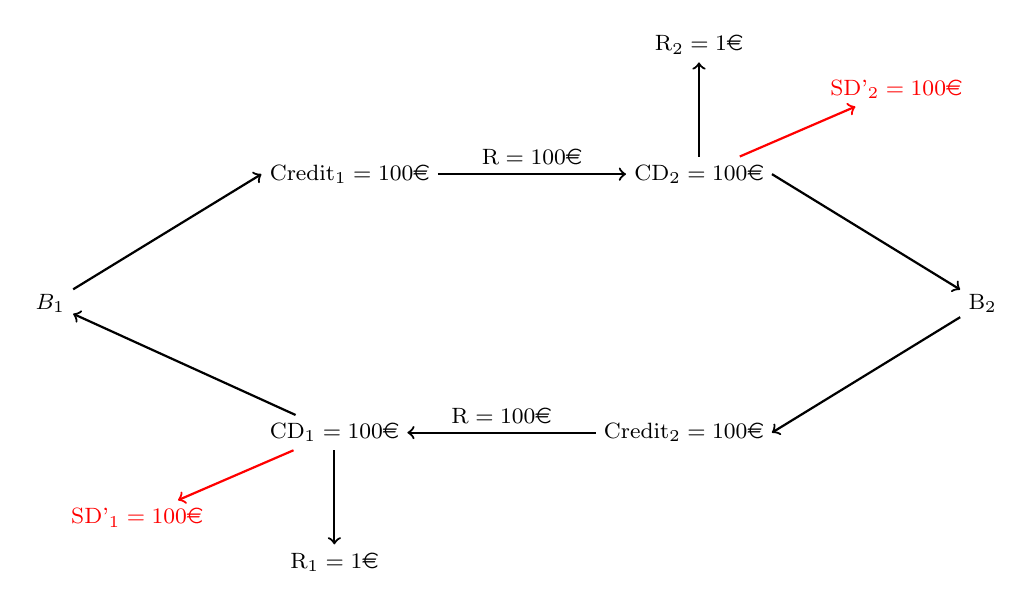
\begin{tikzpicture}[node distance = 4 em and 8em]
\node(B1) at (0,0) {$B_1$};

\node[above right = of B1](cr1){$\text{Credit}_1 = 100 \text{\euro}$};
\node[right = of cr1](cd2){$\text{CD}_2 = 100 \text{\euro}$};
\node[above = of cd2](r1){$\text{R}_2 = 1 \text{\euro}$};

\node[below right = of cd2](b2){$\text{B}_2$};
\node[below left = of b2](cr2){$\text{Credit}_2 = 100 \text{\euro}$};

\node[left = of cr2](cd1){$\text{CD}_1 = 100 \text{\euro}$};
\node[below = of cd1](r2){$\text{R}_1 = 1 \text{\euro}$};

\draw[->, thick] (B1) -- (cr1.west);
\draw[->, thick] (cr1) -- node[pos=0.5,sloped,above]{$\text{R} = 100 \text{\euro}$} (cd2);
\draw[ ->, thick] (cd2) -- (r1);

\draw[->, thick] (cd2.east) -- (b2);
\draw[->, thick] (b2) -- (cr2.east);
\draw[->, thick] (cr2) -- node[pos=0.5,sloped,above]{$\text{R} = 100 \text{\euro}$} (cd1);

\draw[->, thick] (cd1) -- (B1);

\draw[->, thick] (cd1) -- (r2);


\node[right = 6 em of B1](dot1){};
\node[left = 6 em of b2](dot2){};

\node[below = 0.5 em of dot1](dot11){};
\node[below = 0.5 em of dot2](dot22){};


\node[red,above right = 3 em of cd2](sd2){$\text{SD'}_2 = 100 \text{\euro}$};
\draw[thick, red, ->] (cd2) -- (sd2);

\node[red,below left = 3 em of cd1](sd1){$\text{SD'}_1 = 100 \text{\euro}$};
\draw[thick, red, ->] (cd1) -- (sd1);

\end{tikzpicture}

    \caption{Caption}
\end{figure}


$\implies$ profits of each bank = $ i_C \cdot Credit-i_{SD}\cdot SD-i_{CB}\cdot R=3\%(100\text{\euro})-1\%(100\text{\euro})-0=(3\%-1\%)(100\text{\euro})=2\text{\euro}$.

The recipients of the payments will not keep their checking deposits either. They will convert them into savings deposits to get an interest rate, $i_{SD}=1\%$. 

Lessons:
\begin{itemize}
    \item Money (CD) is created as a result of the initiative of HBS to ask for a bank loan. Credit created the deposits. 
    \item Quantity of money in circulation is not fixed by the CB. The CB fixes the $i_{CB}$.
    \item The quantity of money changes when HBS ask for bank credit. Money is endogenous to the economy.
\end{itemize}

\paragraph{When banks extend credit to HBS, say of 103\euro:}
\begin{itemize}
    \item They don't hand 103\euro over; 
    \item They simply open a new checking deposit. 
\end{itemize}

% balance sheets

Two lessons: 
\begin{enumerate}
    \item Credit $\rightarrow$ Deposits; 
    \item The money created and held by HBS does not constitute net wealth for them. 
\end{enumerate}

When HBS who get the credit eventually pay it back in the future, they don't hand 103\euro in notes and coins, they just tell the banks to eliminate their CD's. 

Thus, the payment of bank loan=103\euro, represents the destruction of checkable deposits of 103\euro, which is equal to the destruction of money=103\euro.

\paragraph{How much Reserves does the bank need to back the credit it has extended?}

\begin{figure}[H]
    \centering
    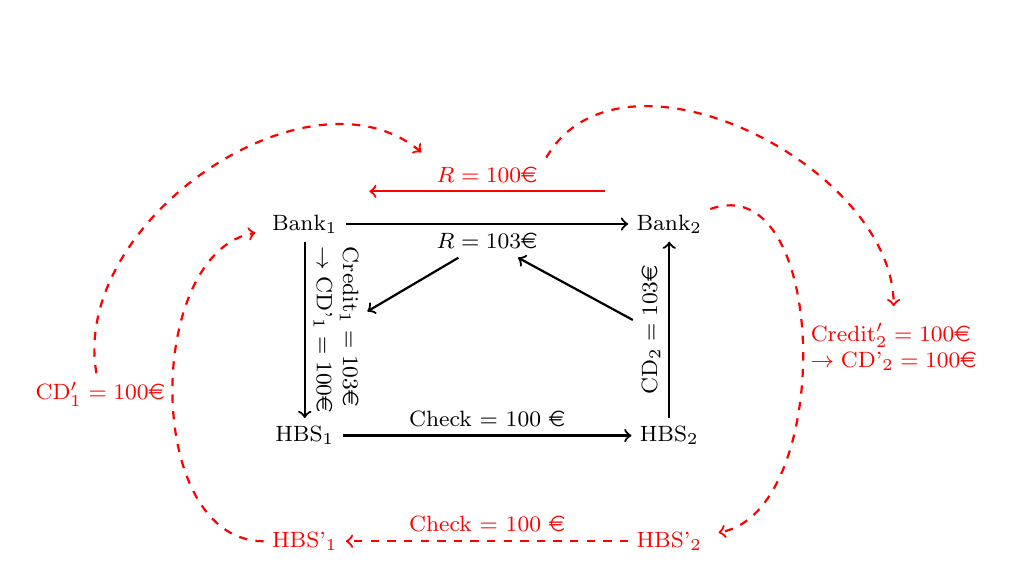
\begin{tikzpicture}[node distance = 3 em]
\node (B1){$\text{Bank}_1$};
\node [right = 12 em of B1](B2){$\text{Bank}_2$};
\node [below =7.5 em of B1](HBS1){$\text{HBS}_1$};
\node [below = 7.5 em of B2](HBS2){$\text{HBS}_2$};

\draw [thick,->] (B1) -- node[pos=0.5,sloped,below](r103){$R = 103 \text{\euro}$} (B2);
\draw [thick,->] (B1) -- node[pos=0.5,sloped,above, align=left](cr11){$\text{Credit}_1= 103 \text{\euro}$ \\ $\rightarrow \text{CD'}_1 = 100 \text{\euro}$} (HBS1);
\draw [thick,->] (HBS1) -- node[pos=0.5,sloped,above]{Check = 100 \euro} (HBS2);
\draw [thick,->] (HBS2) -- node[pos=0.5,sloped,above](cd22){$\text{CD}_2= 103 \text{\euro}$} (B2);







%Red Lines
\node[above left = 0.4 em of B2](B22){}; 
\node[above right = 0.4 em of B1](B11){};
\draw[red, thick, ->] (B22) -- node[pos=0.5,sloped,above](r100){$R = 100 \text{\euro}$} (B11);


\node[red, below = of HBS2](HBS22){$\text{HBS'}_2$};
\node[red, below = of HBS1](HBS11){$\text{HBS'}_1$};

\draw[red, dashed, thick,->,shorten >=3pt] (B2) to [out=20,in=10,loop,looseness=1] node[pos=0.5,right, align=left](cr2p){$\text{Credit}_2' = 100 \text{\euro}$ \\ $\rightarrow \text{CD'}_2 = 100 \text{\euro}$} (HBS22);
\draw[red, dashed, thick, ->] (HBS22) --  node[pos=0.5,sloped,above]{Check = 100 \euro}(HBS11);
\draw[red, dashed, thick,->,shorten >=3pt] (HBS11) to [out=180,in=190,loop,looseness=1] node[pos=0.5,left, align=left](cd1p){$\text{CD}_1' = 100 \text{\euro}$} (B1);

\draw[red, dashed, thick,->,shorten >=3pt] (r100.north east) to [out=60,in=90,loop,looseness=1] (cr2p);
\draw[red, dashed, thick,->,shorten >=3pt] (cd1p) to [out=100,in=140,loop,looseness=1] (r100.north west);

\draw[->, thick] (cd22) -- (r103);
\draw[->, thick] (r103) -- (cr11);

\end{tikzpicture} 

    \caption{Caption}
\end{figure}
At first, $R=1\%(103\text{\euro})=1.03\text{\euro}$

Once $HBS_1$ uses the $CD_1$ to make a payment in favor of costumers of other banks, $R=103\text{\euro}$ (in total). [This is represented by the black arrows]

However, $B_2$ will also extend credit, say of 100\euro. [red arrows]

In sum: 

\begin{figure}[H]
    \centering
    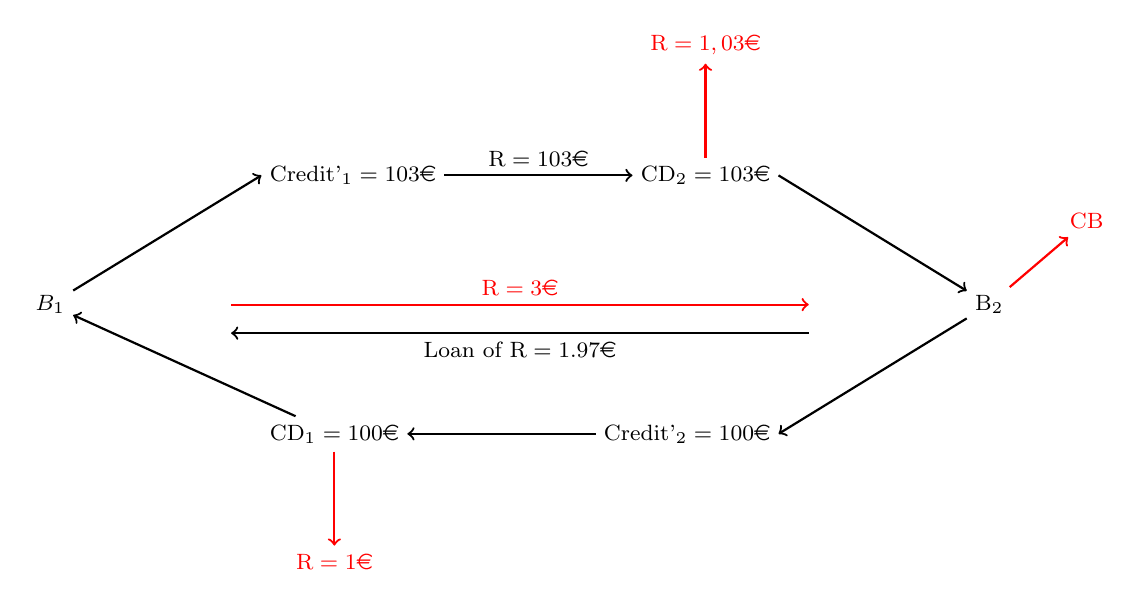
\begin{tikzpicture}[node distance = 4 em and 8em]
\node(B1) at (0,0) {$B_1$};

\node[above right = of B1](cr1){$\text{Credit'}_1 = 103 \text{\euro}$};
\node[right = of cr1](cd2){$\text{CD}_2 = 103 \text{\euro}$};
\node[red, above = of cd2](r1){$\text{R} = 1,03 \text{\euro}$};

\node[below right = of cd2](b2){$\text{B}_2$};
\node[below left = of b2](cr2){$\text{Credit'}_2 = 100 \text{\euro}$};

\node[left = of cr2](cd1){$\text{CD}_1 = 100 \text{\euro}$};
\node[red, below = of cd1](r2){$\text{R} = 1 \text{\euro}$};

\draw[->, thick] (B1) -- (cr1.west);
\draw[->, thick] (cr1) -- node[pos=0.5,sloped,above]{$\text{R} = 103 \text{\euro}$} (cd2);
\draw[red, ->, thick] (cd2) -- (r1);

\draw[->, thick] (cd2.east) -- (b2);
\draw[->, thick] (b2) -- (cr2.east);
\draw[->, thick] (cr2) -- (cd1);

\draw[->, thick] (cd1) -- (B1);

\draw[red, ->, thick] (cd1) -- (r2);


\node[right = 6 em of B1](dot1){};
\node[left = 6 em of b2](dot2){};

\node[below = 0.5 em of dot1](dot11){};
\node[below = 0.5 em of dot2](dot22){};

\draw[->, red, thick] (dot1) -- node[red, pos=0.5,sloped,above]{$\text{R} = 3 \text{\euro}$} (dot2);
\draw[->, thick] (dot22) -- node[pos=0.5,sloped, below]{$\text{Loan of R} = 1.97 \text{\euro}$} (dot11);

\node[red,above right = 3 em of b2](cb){CB};

\draw[thick, red, ->] (b2) -- (cb);

\end{tikzpicture}
    \caption{Caption}
\end{figure}
$B_1$ needs to back it's credit=103\euro with $R=1\text{\euro}+3\text{\euro}$

$\implies$ $B_1$'s profits $=i_C \cdot Credit-i_{CB}\cdot R=3\%(103\text{\euro})-1\%(4\text{\euro})$ 

\paragraph{If at the prevailing $i_{CB}$ banks can easily get tiny amount of reserves they need from the CB, why don't they expand Credit indefinitely to expand profits?}
\begin{enumerate}
    \item Banks are limited by the amount of credit demanded by HBS; 
    \item If HBS start to demand too much credit and banks correspond to that demand, too much credit, and hence, money, too much Demand for goods and services $\implies \uparrow \pi \implies \text{CB will increase } i_{CB} \implies \downarrow D_{Credit} \implies \implies \downarrow Credit, \downarrow Money, \downarrow D_{g+s}$.
    \item Banks have to meet $EqK \geq 10\%$ loan:
\end{enumerate}

% Bank balance sheet scheme

If $D_{credit}=110\text{\euro}$ but EqK=10\euro

$D_{credit}>10\cdot EqK \implies$ either issuance of new stocks to increase EqK to 11\euro or restriction of credit to 100\euro. 

\[ 
CD=100 \text{\euro} \implies \left\{
\begin{array}{l l}
    C=5\text{\euro} \\
    SD=65\text{\euro} \\
    CD=30\text{\euro}
\end{array}
\right.
\]

\paragraph{Q1: How does this affect $B_1$'s profits?}
\paragraph{Q2: Imagine there was a single bank.}


%% Because we have refsection=chapter, this will print all the references in the chapter

\chapter{Static macro: is there a mechanism that ensures that aggregate demand is high enough to deliver full-employment?}


\section{Determinants of the level of aggregate consumption}

\subsection{New Classical School  New Keynesian School}
\begin{itemize}
    \item It's assumed that all households are identical (representative agents)
    \item The consumption behaviour of workers and capitalists are alike. 
    \item The representative agent is able to predict with certainty all his incomes in each and every future years of his life (Perfect Foresight).
\end{itemize}

$C_{t}$ does not depend more on $Y_{t}$ than on $Y_{t+30}$. It depends to the same extent on all incomes of the present, and future years.

For example, if $Y_t<Y_{t+30}$, $C_t$ is not less than $C_{t+30}$. 
The households will gain to borrow in t, to $\uparrow C_{t} \implies \uparrow utility_{t}$ and pay back the loan in t+30 $\implies \downarrow C_{t+30} \implies \downarrow utility_{t}$. 

In sum, $\uparrow utility_t > \downarrow utility_{t+30}$.

Consumption at any point in time depends very little on the income of that time period, but on the average income expected over the lifetime - the so called permanent income. 

So, if people don't want to leave bequests (inheritance), and have perfect foresight:

\begin{equation*}
    C_t=Y_P
\end{equation*}


\subsection{Keynes \heart}

\begin{equation}
    C_t=\overline{C}+cY_t
\end{equation}

Q: Why don't people increase current consumption by borrowing and paying with their future higher incomes, increasing their total utility over the lifetime? 

A: People are uncertain about their future incomes;

\begin{itemize}
    \item People are especially afraid of funding current consumption with loans to be paid with uncertain future incomes; 
    \item Even if they are not, banks will not normally want to provide such funding;
\end{itemize}

$\implies C_t=f(Y_t)$, instead of $C_t=f(Y_t, Y_{t+1}^e, Y_{t+2}^e, ... ,Y_{t+n}^e)$, as in the New Classical, and New Keynesian schools. 

\section{The fundamental question of macro}

\begin{equation*}
    C_t=0.8Y_t
\end{equation*}

Suppose that in a given semester, a country has capital and labour that enables it to produce 100 units of a composite good per month (with price=1 \euro)

\begin{equation*}
    Y_{FC}=100*1\text{\euro}=100\text{\euro} /month
\end{equation*}

Will businesses produce 100 units of the good? Businesses produce according to the demand they receive from their costumers. 

\paragraph{Q:} Is there any mechanism that ensures that $AD=100\text{\euro}$ and, thereby, leads businesses to produce 100 units $\implies FE_{K,L}$.

In a closed economy without government without gov, $AD=C_t^d+I_t^d$

\paragraph{Suppose that, by coincidence, in January $AD_t=100\text{\euro}$}

$$
    AD_t=100 \text{\euro} \implies output_t=100\text{\euro} \implies FE_{K,L}
$$

Note that output equals income, therefore, $output_t=100 \text{\euro} \implies income_t=100\text{\euro} $. When output is sold in t, it generates an income equal to it's full value. 

\begin{equation*}
    Y=output=income=Wages+Interest+Rents+Profits
\end{equation*}

\begin{equation*}
    income_t=100\text{\euro} \rightarrow C_t^d=80\text{\euro} \quad S_{t+1}=20\text{\euro}
\end{equation*}

\paragraph{Q:} Will $AD_{t+1}=100\text{\euro} \implies FE_{K,L}$?

\subsubsection{One possible answer: The Central Bank view}
If (by coincidence) $I_t^d=S_{t+1}=20\text{\euro}$, than, $ \implies AD_{t+1}=80+20=100\text{\euro}\implies Y_{t+1}=100\text{\euro} \implies FE_{K,L}$.

\paragraph{Q:} This may not be the case however. Say, for example, that investment is lower than savings, $I^d_{t+1}=18\text{\euro}<S_{t+1}$. What happens? 

\paragraph{A:} $\downarrow AD_{t+1}$ to $98 \text{\euro} \implies \downarrow output_{t+1}$ to $98\text{\euro}$, below $FE_{K,L}$.

Observing this, the Central Bank will cut interest rates, $\downarrow i \implies I^d_{t+1}$ will quickly rise to 20\euro $\implies AD_{t+1}$ will remain at 100\euro $\implies output_{t+1}=100\text{\euro}=FE_{K,L}$.

\paragraph{Conclusion:} Changes in $i_{CB}$are a mechanism that keeps AD at FE. 

\paragraph{Q:} So, why is unemployment so prevalent in the real world? 

There are two problems with the previous conclusion: 
\begin{itemize}
    \item $\downarrow i_{CB}$ all the way to zero is sometimes not enough to increase investment back to the level at which it guarantees full employment - the Lower Zero Bound problem of Monetary Policy. 
    \item And even if it does, it's unlikely that the investment will quickly react and increase back to 20\euro. Investment is slow to respond to changes in economic conditions in general, and to the interest rate of the Central Bank in particular. 
\end{itemize}

Investment is slow for 4 reasons - because firms need time:
\begin{enumerate}
    \item To know about relatively permanent changes in economic conditions; 
    \item To ponder whether to advance with new investments, which facilities to build, which machines to buy, etc. 
    \item To get bank loans approved, or to implement bond issues.
    \item To obtain construction permits from the state for new buildings. 
\end{enumerate}

%% INSERT A sCHEME HERE %%

\paragraph{Q:} What will be the level of output in February if investment falls to 18\euro
\paragraph{A:} $\downarrow AD_{t+1} \rightarrow 98\text{\euro}$ 

Observing this, the Central Bank will cut interest rates. 

However, cutting rates down to zero may not be enough, and it will take time for investment to respond. 

In Feb: $S-I=2\text{\euro}$
\begin{itemize}
    \item $S=20\text{\euro} \implies$ Banks pay down 2\euro of their debt with the Central Bank $\implies \downarrow M_1=2\text{\euro}$
    \item $I^d=18\text{\euro}$
    \item $C^d=80\text{\euro} \implies \downarrow AD=98\text{\euro} \implies \downarrow output=98\text{\euro}\implies \downarrow income=98\text{\euro}$
\end{itemize}

In March, $S-I=1.6\text{\euro}$
\begin{itemize}
    \item $\downarrow S=19.6\text{\euro} \implies$ Banks pay down 1.6\euro of their debt with the Central Bank $\implies \downarrow M_1=1.6\text{\euro}$
    \item $I^d=18\text{\euro}$
    \item $\downarrow C^d=78.4\text{\euro} \implies \downarrow AD=96.4\text{\euro} \implies \downarrow output=96.4\text{\euro}\implies \downarrow income=96.4\text{\euro}$
\end{itemize}

If $C_t^d$ depended on $Y_P$, rather than on $Y_t$, it would hardly fall.

The economy is going through a shot term recessive spiral: 
\begin{itemize}
    \item $\downarrow M_1=S-I$
    \item $\downarrow S$
    \item $\downarrow income \implies \downarrow C_t^d \implies \downarrow AD \implies Output Sold$
\end{itemize}

When will the recessive spiral end? 

\paragraph{As long as $S>I=18\text{\euro}$}

The $income=output=AD$ of one month leads to a smalled $AD=output=income$ in the following month. 

\paragraph{When $AD=output=income$} 

eventually falls to 90\text{\euro} in May

%In June $\downarrowS=18\text{\euro}=I^d\implies$ in June, $AD=90\text{\euro}=output=income$ (red letters in the scheme).

This would be a steady state characterised by high unemployment. 

A vicious circle: 
\begin{itemize}
    \item Why is there unemployment? Because AD is low ($90\text{\euro}<100\text{\euro}$) \textcolor{green}{was 100 \euro}
    \item Why is AD low? 
    \begin{itemize}
        \item Because $I^d$ is low ($18\text{\euro}\ < 20\text{\euro}$) \textcolor{green}{was 20\euro}
        \item $C^d$ is low ($72\text{\euro}<80\text{\euro}$) \textcolor{green}{was 80\euro}
        \item $C^d$ is low because income is low ($90\text{\euro}<100\text{\euro}$) \textcolor{green}{was 100\euro} and there is unemployment \textcolor{green}{Whereas before there was Full Employment}
    \end{itemize}
\end{itemize}

% Vicious circle scheme



\paragraph{A note:}

$\downarrow I^d$ from 20\euro to 18\euro $\implies \downarrow AD$ from 100\euro  to 90\euro. 

In essence, $\downarrow I^d=2\text{\euro}\implies \downarrow AD=10\text{\euro}$. This is the idea of a Keynesian multiplier. 

Recall the Keynesian system: 
\begin{itemize}
    \item $Y=AD$
    \item $AD=C^d+I^d$
    \item $C^d=0.8Y_t$
\end{itemize}

\begin{equation*}
    \begin{aligned}
        Y=0.8Y+I^d_{-1} \\
        (1-0.8)Y=I^d_{-1}\\
        Y=\frac{1}{1-0.8}\cdot I^d_{-1} \\
        Y=\frac{1}{0.2}\cdot I_{-1}^d
    \end{aligned}
\end{equation*}

$\downarrow I^d=2\text{\euro} \implies \downarrow Y=10\text{\euro}$

\subsection{The effects of increased Savings}
\begin{enumerate}
    \item If you want to increase of consumption tomorrow at the expense of consumption today, all she has to do to is to save some income by accumulating capital (deposits or stocks and bonds). Use the saved money to buy consumption goods in the future, instead of today.
    \item If a country wants to increase consumption tomorrow, at the expense of consumption today, savings is not enough. More consumption tomorrow is only possible if the production capacity is higher, which will only happen when savings leads to investment.  
\end{enumerate}

	Savings must be converted into investments to accumulate capital stock:
	
	$$I\implies \uparrow K \implies \implies \text{More capacity to produce consumption goods tomorrow.}$$


\paragraph{Question} Will an increase in savings will it lead to an increase in investment? The answers will be shown in the context of the previous static model. 

Assuming we start at full employment

%\begin{equation}
 %\text{Income}_t = 100 \euro \rightarrow C^d_{t + 1} \rightarrow AD = 100 \euro \implies 100 \euro = FE, U_L 4%, U_K = 15%
 %\end{equation}
 
 
 \paragraph{Question} If for some reason the savings rate, rises to 22%, what is the effect?

	Savings goes from 20 \euro to 22 \euro, consumption falls from 80 \euro to 78 \euro, therefore demand and thus output falls from 100 \euro to 98 \euro. What happens next? 
	
		Two possibilities:
	
	\subsubsection{The central bank view}
			A quick cut in interest rates, which leads to a rapid increase in investment. From 20 \euro up to 22 \euro, which leads to an increase in AD and Y so it recovers from 98 \euro up to 100 \euro. Notice that 100 \euro is 78 \euro (C) + 22 \euro (I), instead of 80 \euro + 20 \euro. 
			
		\subsubsection{A short summary:} 
An increase in aggregate savings

$$ s \uparrow \implies \uparrow S \implies \downarrow c^d \implies \downarrow AD \implies \downarrow i_{CB} \implies \uparrow I^d \implies \uparrow g_K = \frac{\Delta K}{K} = I_N = \uparrow T_P$$

$$\uparrow g_{PC} = \text{The rate of growth of production capacity}$$

Lower consumption today, but more investment today. An increase in savings alters the composition of output, a reduction in production consumption of goods and an increase in the production of investment goods. It leads to an increase in the growth rate of capital accumulation. 

Another effect, newer machines are better than the others, which leads to an increase in the rate of growth of tech. progress, which in turn leads to more efficient production and more consumption in the future. 

Consumers are worse off today, but better off tomorrow. Sacrificing current wealth in favour of more wealth in the future. 

In the Keynesian view, current consumption is mainly determined by current income. This is contradictory of New Keynesian views.


According to the Keynesian view,
The investment demand is fixed:

$$I^d = 20 \text{\euro}$$

$$\text{AD and Y} = \downarrow 98 \text{\euro}$$

What happens in the following months? 

The next month:

*Income is lower: 98 \euro
*Savings is now: 20\% instead of 98 \euro =
* What happens when savings exceed investments? Recall that savings is income that does not depend on demand. 

$$\text{AD}_{t + 1} < \text{Income}_t = \text{AD}_t$$

\section{The Paradox of Thrift}

Does an increase in savings rate (20\% to 22\%)  lead to an increase in investment? \
\
$$\uparrow s \implies \uparrow S \implies \downarrow C^d \implies \downarrow AD \implies \downarrow Y \text{(income and output)} \implies \downarrow S$$

$$\Delta S = ?$$

$$\Delta Y = ?$$

On one hand people are saving a larger portion of their income, but it leads to to a decrease in demand and thus output and in turn leads to a reduction in total Savings. 

People try to save more, by increasing savings rate, they consume less, lower demand, lower output, lower income, in total lower saving. 

Notice that the recessive spiral ends when savings equal investment again. Meaning that AD has decreased so much that the larger share of saving is equal to the fixed amount of investment. 

Which effect is bigger? They can cancel each other out.

An increase in savings does not lead to an increase in investment, the level of investment is fixed and determined by previous economic conditions. 

Results:
$$\Delta S = \Delta I = \emptyset \implies ?? \uparrow g_{PC}$$


Consumption is lower and income is lower, thus we are worse off by increasing the savings rate in this case. Lower consumption means lower demand, firms produce less and demand less workers, thus we have 2 negative effects and no positive effects in the future. The revenue of the firms fall, less income distributed. 


\begin{figure}[H]
    \centering
        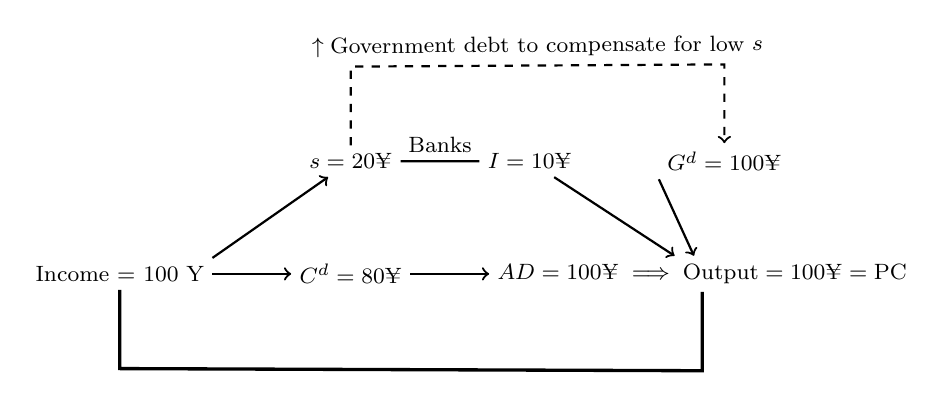
\begin{tikzpicture}
    \node at (0,0) (income){Income = 100 Y};
    \node[right = of income](consumption){$C^d = 80 \text{\yen}$};
        \node[right = of consumption](ad){$AD = 100 \text{\yen} \implies \text{Output} = 100 \text{\yen} = \text{PC}$};
                \node[above = of consumption](s){$s = 20 \text{\yen}$};
                                \node[right = of s](I){$I = 10 \text{\yen}$};
                                                                \node[right = of I](G){$G^d = 100 \text{\yen}$};




    
    \coordinate[below = of income](i_1);
        \coordinate[below = of ad](i_2);

    
    \draw[very thick] (income) -- (i_1) -- (i_2) -- (ad);
    \draw[->,thick] (income) -- (consumption);
        \draw[->,thick] (consumption) -- (ad);
                  \draw[->,thick] (s) -- node[pos=0.5,sloped,above]{Banks}(I) -- (ad);

                

                \draw[->,thick] (income.north east) -- (s);
                                \draw[->,thick] (G.south west) -- (ad);
                                \coordinate[above = of s] (splus);
                                                                \coordinate[above = of G] (gplus);

                                
                                                \draw[->,dashed,thick] (s) -- (splus) -- node[pos=0.5,sloped,above]{$ \uparrow \text{Government debt to compensate for low $s$}$} (gplus) -- (G);




    
    \end{tikzpicture}
    \caption{Caption}
\end{figure}

\section{Secular Stagnation}
Japan has faced a secular stagnation (elaborate) over the past 25 years. There are several reasons for that. 

$$PC = 100 Y$$
$$i_{\text{BoJ}} = 0\%$$

\subsection*{Two reasons for the low levels of private investment}

\begin{enumerate}
    \item A declining population due to a low fertility rate. This has lead to a low demand for new housing because new generations will inherit from their parents. The consequence is that real estate investment has been very low in the last 25 year period. 
    \item A declining working-age population has led to a shriking of the workforce. Low investment in mch, capital. 
nking of the wiro kofce, ardnin  utnrhas crea t\end{enumerate}


With $G^d = \emptyset$, aggregate demand would go down to 50\yen ($\downarrow \text{AD} = 50 \yen$). In turn income would also go down to 50\yen, savings would go down to 10. $S = 10 \yen = I^d$. Unemployment would increase to hiugher levels. 

However, since the government increased their spendings, Japan has been able to soften the recessive effects of the demographic situation:

$$G^d = 10 \yen = S = I$$

This led to AD being kept at 100 \yen, which is max production capacity which ensured full employment. However, government debt grew from 67\% of GDP in 1995 to 250\% of GDP as of today.


\chapter{Static macro: Kalecki’s variant of Keynesian economics}

\section{Price Determination}

\begin{figure}[H]
    \centering
        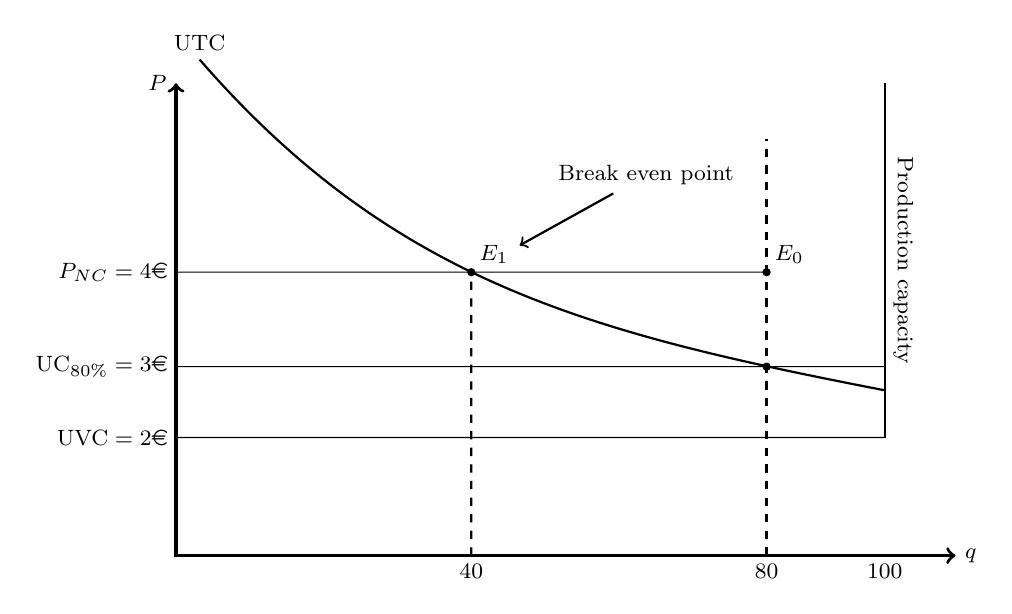
\begin{tikzpicture}[scale = 3]
    % Draw axes
    \draw [<->, very thick] (0,2) node (yaxis) [left] {$P$}
        |- (3.3,0) node (xaxis) [right] {$q$};
    \node at (0.5,0)(lf){};
    \node[below] at (2.5,0) (80){80};
    \node[below] at (3,0) (100){100};
   \node[below] at (1.25,0) (40){40};
    \node at (2.5,1.8) (point){};
   \coordinate (low_profit) at (2.5, 0.5);
      \coordinate (med_profit) at (2.5, 0.8);
            \coordinate (high_profit) at (2.5, 1.20);
                        \coordinate (e1) at (1.25,1.20);
            \node[above right] at (e1) {$E_1$};
            \fill[black] (e1) circle (0.5pt);
                        \node[above right = of e1] (br) {Break even point};
			 \draw[->, shorten >=20pt, thick] (br) -- (e1);
                        \fill[black] (high_profit) circle (0.5pt);
                                    \node[above right] at (high_profit) {$E_0$};
                                                            \fill[black] (2.5,0.8) circle (0.5pt);
   \draw[dashed, thick] (80) -- (point);
      %\draw[dashed, thick] (40) -- (point);
\coordinate (p1) at (0, 1.25);
\draw (high_profit)  --  (0, 1.20) node [left] {$P_{NC} = 4\text{\euro}$};
\draw   (0, 0.8)  node [left] {$\text{UC}_{80\%} = 3\text{\euro}$} -- (med_profit) -- (3,0.8);
\draw (0, 0.5) node [left] {$\text{UVC}= 2\text{\euro}$}    -- (low_profit) -- (3,0.5);
\draw[thick] (0.1, 2.1) coordinate (utc_1) node[above]{UTC} to [out=311,in=169] (3,0.7) coordinate (utc_2);
      \draw[dashed, thick] (40) -- (1.25,1.20);
      \draw[thick] (3,0.5) -- node[pos=0.5,sloped,above, rotate = 180]{Production capacity} (3,2);
    \end{tikzpicture}
    \caption{Caption}
\end{figure}


\paragraph{Keynesian idea:} AD may determine a level of output below full employment. 

A slightly different version of the same model. 

The main difference is that Kalecki said income distribution affects the ... The propensity to consume (In OECD countries about 90%, which is well above the $c$ out of profits?). 

$D$ denotes profits. 

1. Determination of income distribution between aggregate wages, profits, rents, interest income 

Understanding income distribution, we need to know how firms set their prices. 

\textbf{Two types of workers:}
\begin{itemize}
	\item Those whose number varies in the same proportion with the level of output: Production line workers: $$W_v$$
	\item Workers who are needed in a roughly fixed quantity, regardless of the level of output (Overhead workers): $$W_f$$ 
\end{itemize}
\section{Price Determination}
Two types, fixed and variable
Fixed Costs $f = R_f + I_f + W_f = 80 \text{\euro}$

\textbf{Variable costs:} Raw materials, energy, and production line workers: $$UVC = E_m + RM + w_v =2 \text{\euro}$$

Unit total cost curve (UTC):\
What happens to UTC when UTC = 100

The fixed costs are shared between more meals, thus the fixed unit costs per meal decreases. 

As $\uparrow q$ to full capacity, the fixed cost is spread over more and more meals $\implies \downarrow UFC \implies \downarrow UTC$. 

\begin{itemize}
    \item If $q=1 \implies UFC=80\text{\euro}$;
    \item If $q=80 \implies UFC=1\text{\euro}\implies UTC=3\text{\euro}$;
    \item If $q=40 \implies UFC=2\text{\euro}\implies UTC=4\text{\euro}$
\end{itemize}

% Price determination and income distribution graphs

\paragraph{The normal rate of utilisation} 

The typical restaurant wants to have on average, over time, some idle seats. Let's say, 20 in 100 seats, i.e, some spare capacity. Why? To meet occasional increases in demand and thus never be forced to turn costumers down. This is crucial in the case of both: 

\begin{description}
    \item New costumers: to avoid losing the opportunity of conquering new costumers; 
    \item Regular costumers: to avoid losing their good will, and, eventually, them.
\end{description}

\paragraph{How does the firm set it's price?}

\begin{enumerate}
    \item They calculate the UC if sales lead to a production equal to 80\% of their capacity: $UC_{80\%}=3\text{\euro}=\text{Normal unit costs}$. 
    \item They add a margin so as to obtain a certain target profit rate if production ends up at the normal level (80\% of FC).
\end{enumerate}

Ex: 

$$
P_{NC}=3\text{\euro}+1\text{\euro}=UC_{80\%}+Umg=
80\cdot1\text{\euro}=80\text{\euro}=\text{Target Profits}\implies\text{Target Profit Rate}
$$

$$
\text{Profit Rate}=\frac{80 \text{\euro}}{800 \text{\euro}}
$$

Where the 800\euro is initial investment. 

\subsubsection{Income Distribution}

\paragraph{A. The distribution of aggregate income if D=80 meals=320\euro}

$\implies$ Aggregate income is divided in 4 equal shares

\paragraph{B. What may lead to changes in that income distribution?}

\begin{enumerate}
    \item If many markets cease to be competitive and become monopolistic or oligopolistic, firms will be able to aim at higher profit rates, say, 20\% instead of the previously assumed 10\%. Result:
    \begin{description}
       \item $\uparrow \text{Umg from 1\euro to 2\euro} \implies \uparrow \text{Profits from 80\euro to 160\euro}$
       \item $\uparrow P_{NC} \text{from 4\euro to 5\euro} \implies \uparrow\text{Aggregate nominal income from 320\euro to 400\euro}\implies $
       \item $\implies \uparrow \text{share of profits 25\% to 40\%}$
    \end{description}
    \item If unions impose $\uparrow W_N$ for production line workers of 100\%
    \begin{description}
        \item The result: $\uparrow W_V$ from 1\euro to 2\euro $\implies \uparrow UC_{80\%}$ from 3\euro to 4\euro $\implies \uparrow P_{NC}$ from 4\euro to 5\euro 
            \begin{description}
                \item $\implies$ Profits remain=80\euro
                \item $\implies$ Profits rate remains=10\%
            \end{description}
        \item $\uparrow W_V$ from 80\euro to 160\euro
        \item F remains=80\euro 
        \item Profits remain=80\euro
        \item RM+Em=80\euro
        \item $\implies \uparrow$ Share of $W_V$ at the expense of everybody else.
    \end{description}
    \item If $\uparrow AD$ as in economic expansions 
        \begin{description}
            \item For each $\uparrow AD=1unit=4\text{\euro}=P_{NP}$:
            \begin{description}
                \item $\uparrow output=1 \implies \uparrow L_V=1 \implies W_V=1\text{\euro}$
                \item $\uparrow$ Cost in RM+Em=1\euro
                \item $\Delta F=0$
                \item $\uparrow$Revenues=4\euro=Ag. Income
            \end{description}
            \item $\implies Profits=2\text{\euro}$
        \end{description}
\end{enumerate}

So, $\uparrow AD=x\% \implies$
\begin{itemize}
    \item $\uparrow W_V=x\% \implies \frac{W_V}{Y}$ is constant; 
    \item $(R_f+I_f+W_f)$ constant $\implies \downarrow \frac{F}{Y}$;
    \item $\uparrow Profits=2x\% \rightarrow \downarrow$share of F in favour of the share of profits in Aggregate Income. 
\end{itemize}


\section{Determinants of the level of aggregate consumption according to Kalecki}

Keynes: 
$$C^d = \bar{C} + cY$$

Kalecki:
$$C^d = C^d_w + C^d_p$$


$$C^d = \bar{C}^d_w + c_w W + \bar{C}_p^d + c_p P$$

Simplifying the Kaleckian consumption functions: 

1. $c_w = 1$ – Propensity to consume out of wages is 1, and thus all wages is spent on consumption.

$$C^d = W + \bar{C}^d_p + c_p P$$

2. $c_p = \emptyset$ and $c_w = 1$

$$C^d = W + \bar{C}_p^d$$

An important implication of using the Kalecki function vs. the Keynesian (Closed, no gov):

Suppose the production capacity is 100 \euro:

$Y_{PC} = 100 * 1 \text{\euro}$, net income: 90 \text{\euro}, $C = 0.8Y$, $\bar{I}^d = 18 \text{\euro}$

Income in t is 90 \euro, consumption is 72 \euro, investment is 18 \euro, 

Then AD=?

%Scheme goes here 

If $\uparrow \overline{I}^d=2\text{\euro}\implies \uparrow AD=2\text{\euro} \implies \uparrow Output=\uparrow income=2\text{\euro} \implies \text{in Feb} \uparrow C^d=0.8\cdot2\text{\euro} \implies \uparrow AD=1.6\text{\euro} \implies ... \implies \uparrow \text{Total Output}=10\text{\euro}$

\subsection{Keynesian output determination}
\[ 
\left\{ \begin{array}{l} 
AD = Y \\
I^d = \bar{I}^d_{-1} \\
C^d = \bar{C} + cY
\end{array} \right.
\]

\paragraph{Reduced form}
\begin{equation}
\begin{aligned}
        AD \rightarrow Y \\
        \bar{C}+cY+\bar{I}^d_{-1}=1\cdot Y \\
        \bar{C} + \bar{I}^d \cdot 1 = (1 - c)Y \\
        Y=\frac{1}{s}(\bar{C}+\bar{I}^d_{-1})
\end{aligned}
\end{equation}

This is the Keynesian multiplier.

\subsection{Kaleckian output determination}
\[ 
\left\{ \begin{array}{l} 
AD = Y \\
I^d = \bar{I}^d_{-1} \\
C^d = W+\bar{c}_p+c_p\cdot P \\
Y=W+P
\end{array} \right.
\]

\[ 
Y=
\left\{ \begin{array}{l l}
    P & \pi=\frac{P}{Y} \implies \pi \cdot Y=P \rightarrow \text{profit share} \\
    W  &
\end{array} \right
.\]

\begin{equation}
\begin{aligned}
    AD \longrightarrow Y \\
    W+\bar{C}_p+c_p\cdot P+\bar{I}^d_{-1}=W+P \\
    \bar{I}^d_{-1}+\bar{C}_p+c_p\cdot P=P \\
    \bar{C}_p+\bar{I}^d_{-1}=(1-c_p)\cdot P \\
    \bar{C}_p+\bar{I}^d_{-1}=s_p \cdot \pi \cdot Y  \\
    \frac{1}{s_p \cdot \pi}(\bar{C}^d_p+\bar{I}^d_{-1})=Y
\end{aligned}
\end{equation}

This equation gives the kaleckian multiplier, which, depends on income distribution, unlike the keynesian multiplier. 

Three reasons why $c_w>c_p$: 
\begin{enumerate}
    \item Capitalists have higher incomes $\implies$ less motivation to increase consumption when their income rises. 
    \item Profits fluctuate a lot over the business cycle.
    \begin{description}
        \item This is because a big, if not the major part, of a companies cost is fixed, $F=R_f+W_f+I_f$. 
        \begin{description}
            \item Thus: $\downarrow$ sales in a recession $\implies \downarrow Revenues > \downarrow Costs \implies \downarrow \text{amplified Profits}$; 
            \item $\uparrow$ sales in an expansion $\implies \uparrow Revenues>\uparrow Costs \implies \uparrow \text{amplified Profits}$
            \item It makes sense not to $\uparrow C_p$ in expansions in order to not be forced to $\downarrow C_p$ in recessions.
            \item i.e. $C_p=f(permanent income)$ and not $f(current income)$
        \end{description}
    \end{description}
    \item Capitalists return from saving is higher
    \begin{description}
        \item Worker's savings are usually applied in a savings deposit $\implies$ the return is very low after taxation; 
        \item Capitalists can reinvest their savings in their business; 
        \item The more capitalists reinvest their savings, the more they can borrow to fund investment projects.
    \end{description}
\end{enumerate}

There are three reasons why the more a capitalist reinvests his profits, the more he can borrow to fund investment projects: 
\begin{enumerate}
    \item The use of his own funds to finance investment is a signal to creditors that he really believes that the investment will bring satisfactory returns, and, as a result, he will be able to repay the loan. 
    \item When investment goods, machines for ex, are purchased with borrowed money, they are often used as collateral for the loan. Thus, if Mch=3M\euro is bought: 
    \begin{description}
        \item With a loan=3M\euro because the machine depreciates over time, it's value will be insufficient to provide a full guarantee for the loan. 
        \item With a loan=1.5M\euro, creditors can, if necessary, sell the machine in the secondary market to get the full loan repaid. 
        \item Conclusion: Creditors require companies to put part of the funds to invest $\implies$ The more capitalists reinvest their savings out of profits, the more loans they can take. 
    \end{description}
    \item $\uparrow \frac{debt}{asset}\implies \frac{\text{debt obligations}}{CF}\implies \uparrow \text{probability of default} \implies \downarrow \text{willingness to invest}$
\end{enumerate}

To understand this, consider the balance sheet of a company:

% Balance sheet of a firm taking a loan 

Note that debt imposes the firm fixed obligations in the form of interest payments, and amortisations. 

Assets, on the other hand, generate uncertain cash flows.

$CF=P\cdot Q-VarCosts-Rents-OverheadSalaries$.

$Profits=CF-InterestPayments$.

Now: 
\begin{description}
    \item If debt=100\euro $\implies$ debt obligations=10\euro $\implies$ The Return on Assets (ROA) must be $\geq 10\%$ to generate a CF high enough for companies to meet their debt obligations, $10\%\cdot100\text{\euro}$. 
    \item If debt=1\euro $\implies 0.1\text{\euro} \implies$ The ROA can drop to 0.1\% and enough CF will still be generated to meet their debt obligations. 
\end{description}

\section{Determination of the level of employment: Keynes vs Kalecki}
\section{Closed economy without government: capitalists earn what they spend}

Workers spend all they earn, while capitalists earn what they spend (in a closed economy without government). 

\paragraph{1.}
\begin{equation*}
    \begin{aligned}
        AD=Y \\
        C_w^d+C_p^d+\bar{I}^d_{-1}=W+P \\
        C^d_p+\bar{I}^d_{-1}=P
    \end{aligned}
\end{equation*}

The value of capitalists expenditures determines and is equal to the value of their profits, i.e, capitalists earn what they spend.

Meanwhile, workers spend what they earn: $C^d_w=W$.

\subsection{The first way of understanding why}

\begin{figure}[H]
    \centering
       \tikzset{block1/.style={shape=rectangle, draw, node distance=-1pt, minimum width = 4em, minimum height = 3 em, line width=1pt}}
    \begin{tikzpicture}[scale = 1.5]
        \node[block1] (P) {P};
        \node[block1,below=of P](W) {W};
        
       
	\draw[decorate, decoration={brace,amplitude=10pt}] (P.north east) -- (P.south east) node [black,midway, right, xshift = 1 em] {$50 \text{\euro} \leftarrow \Bar{C}_p^d + \Bar{I}_{-1}^d$};
		\draw[decorate, decoration={brace,amplitude=10pt}] (W.north east) -- (W.south east) node [black,midway, right, xshift = 1 em](W1) {$50 \text{\euro}$};
		\node[right =  3em of W1]{$C^d_w$};
		
		\draw[dashed, thick,->,shorten >=1pt] (W1.south) to [out=300,in=20,loop,looseness=8]  ( W1.north east);
	\draw[decorate, decoration={calligraphic brace,amplitude=10pt, mirror}, line width=1pt] (P.north west) -- (W.south west) node [black,midway, left, xshift = -1 em] {$Y = 100 \cdot 1 \text{\euro}$};

    \end{tikzpicture}
    \caption{Profit and consumption flows}
\end{figure}

The total amount of wages paid by firms is entirely spent to buy consumption goods from those firms $\implies$ it generates revenues only high enough for firms to cover their wage costs. 

% First scheme with the squares 

Any revenue beyond those wage costs (i.e. profits) must come from capitalists' expenditures. 

\subsection{Second way}

\begin{figure}[H]
    \centering
    \tikzset{block/.style={shape=rectangle, 
        draw, 
        minimum width = 4em, 
        line width=1.2pt
                }}

    
    \begin{tikzpicture}[scale = 2]


%Firm 1
\node[block, rectangle split, rectangle split parts=2, draw] (f1) 
       {{$P_1$}
        \nodepart{two} $W_1$};
        
  \node[above of = f1] (mch) {Machines (1)};
  \node [above right = 1.5 em and 0.2 em of mch] (kists){Capitalists};
  \draw [->, thick] (kists.south) -- (mch.north east);
 


%Firm 2
\node[block, rectangle split, rectangle split parts=2, draw, right = 2 cm of f1] (f2) 
       {{$P_2$}
        \nodepart{two} $W_2$};
          \node[above of = f2] (hotel){Hotel Services (2)};
             \draw [->, thick] (kists.south) -- (hotel);
          
          
          %Firm 3
\node[block, rectangle split, rectangle split parts=2, draw, right = 2 cm of f2] (f3) 
       {{$P_3$}
        \nodepart{two} $W_3$};
          \node[above of = f3](bread) {Bread (3)};
          \node[above of = bread](workers){Workers};
          \draw[->, thick] (workers) -- (bread);


\draw[dashed, ->, thick] (f1.two east)-- node[pos=0.8,sloped,above]{(1)} (f3.north west);
\draw[dashed, ->, thick] (f2.two east)-- node[pos=0.5,sloped,below]{(2)} (f3.north west);

		\draw[dashed, thick,->,shorten >=3pt] (f3.two south) to [out=300,in=0,loop,looseness=6]  node[pos=0.8,sloped,above]{(3)}( f3.two east);
		
		
		%Investment and capitalist demand
		\node[above right = of f2, red] (cdp) {$\Bar{C}_p^d$};
		\draw[dashed, ->, thick, red] (cdp)--(f2.north east);
		\node[above left = of f1, red] (idp) {$\Bar{I}_{-1}^d$};
		\draw[dashed, ->, thick, red] (idp)--(f1.north west);




\end{tikzpicture}

    \caption{Caption}
\end{figure}
\paragraph{a)} The profits of the bread sector cannot come from the expenditure of the workers of that sector: 

Their expenditure generates revenue only high enough to pay the wages of their workers. 

Can only result from expenditure of workers of the other two sectors, i.e, $P_3=W_1+W_2$.

The wages of workers of sectors (1) and (2) determine and are equal to the profits of the bread sector. 

\paragraph{b) What determines $W_1+W_2$?}

They're a share (say 50\%) of the total income distributed by those sectors. 

\paragraph{c) The chain of causality:}

\begin{equation*}
    \begin{aligned}
        \bar{I}^d_{-1}+\bar{C}_p^d=P_1+P_2+ \text{(directly)} \\
        +W_1+W_2 \rightarrow P_3 \text{(indirectly)}
    \end{aligned}
\end{equation*}

Ergo, $\bar{I}^d_{-1}+\bar{c}_p^d=P_1+P_2+P_3$.

\paragraph{4. Third way}. 

Start from $Y=90\cdot 1\text{\euro}<Y_{FC}=100\cdot 1\text{\euro}$

Note, $Y=90\cdot 1\text{\euro} \rightarrow L=45 < L^S=50 \leftarrow Y_{FC}=100 \cdot 1\text{\euro}$.

Assume that $\pi=0.5$, meaning $P=45$\euro and $W=45$\euro and $C^d_p=\bar{C}^d_p$.

Say a capitalist goes on a luxurious hotel for vacation, 
\paragraph{First:}

\begin{multline}
    \uparrow\bar{C}^d_p=5\text{\euro} \implies \\
\uparrow AD=5\text{\euro} \implies \uparrow Y=5\text{\euro} \And \uparrow L=2.5 \implies \left\{ \begin{array}{r}
    \uparrow W_N = 2.5 \text{\euro}\implies ... \implies \uparrow P_B=2.5\text{\euro} \\ \uparrow P = 2.5 \text{\euro}
\end{array} \right\}
\end{multline}

The reason: one capitalists expenditure is another ones revenue. Half of which is profits, the other half is wages, entirely spent on consumption.

\paragraph{Second:}

\begin{multline}
\uparrow W=2.5\text{\euro} \implies \uparrow C^d_W=2.5\text{\euro} \implies \left\{\begin{array}{r}
     \uparrow Y=2.5\text{\euro} \\
      \uparrow L=1.25
\end{array} \right\} \implies \left\{\begin{array}{r}
     \uparrow P=1.25\text{\euro}  \\
      \uparrow W_N=1.25\text{\euro}
\end{array} \right\}
\end{multline}

Capitalists earn half of what workers spend on bread, because worker's expenditure is capitalists' revenue (bread capitalists in this case).

Half of which is profits, and the other half is wages, entirely spent on bread. 
\paragraph{Third}

\begin{multline}
    \uparrow W_N=1.25\text{\euro} \implies \uparrow C^d_W=1.25\text{\euro} \implies \left\{\begin{array}{r}
        \uparrow Y=1.25\text{\euro}  \\
        \uparrow L=0.625  
    \end{array} \right\} \implies 
    \left\{\begin{array}{r}
         \uparrow P=0.625 \text{\euro} \\
         \uparrow W=0.625\text{\euro} 
    \end{array} \right\}
\end{multline}

In sum: 
\begin{align}
    \uparrow C^d_p=5\text{\euro} \implies \left\{\begin{array}{rr}
        \uparrow P^d_H=2.5 \text{\euro} & \frac{1}{2}\uparrow\bar{C}^d_p  \\
        \uparrow P^d_B=1.25\text{\euro} & \frac{1}{4}\uparrow \bar{C}^d_p \\
        \uparrow P_B=0.625\text{\euro}  & \frac{1}{8}\uparrow \bar{C}^d_p \\
        ... \\
        \sum \uparrow P=5\text{\euro}
    \end{array} \right\}. \end{align}

However much capitalists spend on consumption, their wealth remains the same as before (Keynes).

\section{How the level of aggregate profits is determined in an open economy with government}

\subsection{Open economy without government}


\paragraph{a)}

$AD = Y$ up until full employment.

\begin{equation}
 \Bar{C}^d_w +  \Bar{C}^d_p + \Bar{I}_{-1}^d - M^d + \Bar{X}^d = W + P
\end{equation}

Notice that it's assumed that $M^d = \emptyset$, and that $\Bar{C}^d_w$ and $W$ on the right side cancel each other out (because of the assumption of marginal rate of consumption out of wages=1). 

\begin{equation}
    \Bar{C}^d_p + \Bar{I}_{-1}^d + \Bar{X}^d = P %= \Pi \cdot Y
\end{equation} \label{eq.1}

Profits are not only determined by $\Bar{C}^d_p + \Bar{I}_{-1}^d$, but also $\Bar{X}^d$ and exceed $\bar{C}^d_p+\bar{I}^d_{-1}$ by the exact amount of $X^d$.

The reason:
\begin{itemize}
    \item The wages paid out by firms are entierly used to buy consumption goods from those firms. 
    \item They generate revenue only high enough for firms to recover their wage costs. 
    \item Any extra expenditure - $\bar{C}^d_p+\bar{I}^d_{-1}+\textcolor{red}{X^d}$ - leads to revenue beyond wage costs.
\end{itemize}

\begin{figure}[H]
    \centering
       \tikzset{block1/.style={shape=rectangle, draw, node distance=-1pt, minimum width = 4em, minimum height = 3 em, line width=1pt}}
    \begin{tikzpicture}
        \node[block1] (P) {P};
        \node[block1,below=of P](W) {W};
                \node[block1, red, below = of W](red){\tiny RM + E};
                
	                \node[block1, red, below right = -4.7 em and 10 em of red](red2){$P$};
	                      \node[block1, red, below = of red2](red3){$W$};


       \draw[red, thick, ->] (red) -- (red2.south west);
	\draw[decorate, decoration={brace,amplitude=10pt}] (P.north east) -- (P.south east) node [black,midway, right, xshift = 1 em] {$50 \text{\euro} \leftarrow \Bar{C}_p^d + \Bar{I}_{-1}^d + \Bar{X}^d$};
		\draw[decorate, decoration={brace,amplitude=10pt}] (W.north east) -- (W.south east) node [black,midway, right, xshift = 1 em](W1) {$50 \text{\euro}$};
		
		\draw[dashed, thick,->,shorten >=1pt] (W1.south) to [out=300,in=20,loop,looseness=8]  ( W1.north east);
	\draw[decorate, decoration={calligraphic brace,amplitude=10pt, mirror}, line width=1pt] (P.north west) -- (W.south west) node [black,midway, left, xshift = -1 em] {$Y = 100 \cdot 1 \text{\euro}$};

    \end{tikzpicture}
    \caption{Caption}
\end{figure}


COMMENTED SHIT
% \begin{multline*}
%     \uparrow X^d=100\text{\euro} \implies \left\{\begin{array}{r}
%          \uparrowP_X=50\text{\euro}  \\
%          \uparrow W_X=50\text{\euro} 
%     \end{array}\right\} \implies C^d_W=50\text{\euro} \implies \\ \left\{\begin{array}{r}
%          \uparrow P_W=25\text{\euro}  \\
%          \uparrow W_W=25\text{\euro}  \implies \uparrow C^d_W=25\text{\euro} 
%     \end{array} \right\} \implies \\ \implies \left\{\begin{array}{r}
%           \uparrow P_W=12.5\text{\euro} \\
%           \uparrow W_W=12.5\text{\euro}  \implies \uparrow C^d_W=12.5\text{\euro} 
%     \end{array}\right\} \implies ... \\ ... \implies 
%     \sum \uparrow P_W=50\text{\euro}
% \end{multline*}


\subsection{Effect of increased exports}

\paragraph{b)} The effect of $\uparrow \bar{X}^d=100\text{\euro}$ on output and profits, if $\pi=\frac{P}{Y}=0.5$.

With $\left\{\begin{array}{cc}
      \bar{C}^d_p+\bar{I}^d_{-1} & \text{ Fixed in the short term}\\
      C^d_W=W \\
      Y & \text{ Below full employment}
\end{array}\right.$


\begin{align*}
\uparrow X^d = 100 \text{\euro} \implies \left\{ \begin{array}{r}
    \uparrow P_x = 50 \text{\euro} \\ \uparrow W_x = 50 \text{\euro}
\end{array} \right\} 
\\
 \implies  \uparrow C^d_w = 50 \text{\euro} \implies \left\{ \begin{array}{r}
    \uparrow P_x = 25 \text{\euro} \\ \uparrow W_x = 25 \text{\euro}
\end{array} \right\} 
\\
\implies \uparrow C^d_w = 25 \text{\euro} \implies \left\{ \begin{array}{r}
    \uparrow P_x = 12.5 \text{\euro} \\ \uparrow W_x = 12.5 \text{\euro}
\end{array} \right\}
\\
\implies \uparrow C^d_w = 12.5 \text{\euro} \implies \left\{ \begin{array}{r}
    \uparrow P_x = 6.25 \text{\euro} \\ \uparrow W_x = 6.25 \text{\euro}
\end{array} \right\} \\
\vdots 
\\
\sum \uparrow P_w = 50 \text{\euro}^* = \sum \uparrow W_w
\end{align*}

\begin{equation*}
    \uparrow Y=\uparrow X^d+\uparrow C^d_W = 200 \text{\euro}
\end{equation*}

The reason: 

The 25\euro of the $C^d_W=50\euro$ that do not generate profits directly are spent by workers and end up leading to an increase in profits indirectly, and so on until the increase in consumption is completely absorbed by Profits. 

\paragraph{c)} What if $\pi=\frac{P}{Y}=0.25$, $\frac{W}{Y}=0.75$? 

$\downarrow \pi \implies$ the bigger the effect of $\uparrow X^d$ on $W_X \implies$ the bigger the effect of the increase in exports on the wage goods sector ($C_W$), and thus on the production of wage goods. 

% scheme with lower profits

\paragraph{d)} Given that $P=\pi \cdot Y$ \ref{eq.1} leads to:

\begin{equation*}
    \bar{C}^d_p+\bar{I}^d_{-1}+\bar{X}^d=P \implies \bar{C}^d_p+\bar{I}^d_{-1}+\bar{X}^d=\pi Y \implies Y=\frac{1}{\pi}\big(\bar{C}^d_p+\bar{I}^d_{-1}+\bar{X}^d\big)
\end{equation*}

Hence, $\uparrow \bar{X}^d \implies \uparrow Y=\frac{1}{\pi}\cdot \uparrow \bar{X}^d$

.....



What if $\Pi = \frac{P}{Y} = 0,25$ and $\frac{W}{Y} = 0,75$

\subsection{Closed economy with government}

\paragraph{a)} $AD=Y$

\begin{equation*}
    \bar{C}^d_W+\bar{C}^d_W+\bar{I}^d_{-1}+G^d=W+P+T 
\end{equation*}

\begin{equation}
    \bar{C}^d_p+\bar{I}^d_{-1}+G^d-T=P \text{ Assuming T=0} \implies \bar{C}^d_p+\bar{I}^d_{-1}+G^d=P
\end{equation} 

Profits determined by capitalists' expenditure pus government spending. Profits exceed capitalists' expenditure by the exact value of $G^d$. 

The reason: 

% governement box scheme

\subsection{Open economy with government}
\begin{equation*}
    AD=Y
\end{equation*}
\begin{equation*}
    C^d_W+\bar{C}^d_p+\bar{I}^d_{-1}+G^d-M^d+X^d=W+P+T
\end{equation*}
\begin{equation}
    \big(\bar{C}^d_p+\bar{I}^d_{-1} \big)+\big(G^d-T \big)+ \big(X^d-M^d \big)=P
\end{equation}

The profits of capitals will be increased by the total amount of any trade surplus and budget deficit (begin decreased by a trade deficit or by a budget surplus).

\section{The Paradox of profits}
\subsection{Closed economy without government}

$$
AD=Y
$$
$$
C^d_W+C^d_p+\bar{I}^d_{-1}=W+P
$$
$$
C^d_p+\bar{I}^d_{-1}=P
$$

\subsection{The paradox of profits}

Suppose that, as happened in Portugal in 2011-2013, 
\begin{itemize}
    \item $\downarrow U$ benefits in value and duration; 
    \item $\downarrow$ salaries of public sector workers (10\% in 2011, 15\% in 2013);
    \item The firing of Private sector workers became easier. 
    Ex: lay-off compensation went down from 1 month times nr of years in the company to $\frac{2}{5}$ month times nr of years in the company. 
    \item High unemployment (22.5\% in Dec, 2012).
\end{itemize}

$\downarrow W_N \implies $ in each 1\euro of sales, $\downarrow$ share of wages in favor of the share of profits: 

% scheme on the variation of profits=0 -> paradox of profits



\subsection{Open economy with government}

\paragraph{a)} $AD=Y$

\begin{equation*}
    C^d_W+C^d_p+\bar{I}^d_{-1}+\textcolor{red}{G^d-M^d+\bar{X}^d}=W+P\textcolor{red}{+T}
\end{equation*}

By defining $\textcolor{red}{T=t\cdot Y}$, and $\textcolor{red}{M^d=m\cdot Y}$:

\begin{equation}
    \big(C^d_p+\bar{I}^d_{-1} \big)+\textcolor{red}{\big(G^d-t\cdot Y \big)}+\textcolor{red}{\big(\bar{X}^d-m\cdot Y \big)}=P
\end{equation}

% Scheme of profit variation being positive 

\chapter{Dynamic macro}

\section{Growth of production capacity if $Y \equiv Y_{FC}$}

Assumption 1: $Y \equiv Y_{FC}$
Assumption 2: Unlimited supply of $L$

Then $g_{PC} = g_K$. The reason for this is $Y_{FC} = aK$. $a$ is the productivity of capital. It's been roughly constant since 1954 because technological progress increases the production per worker, but leaves production per capital unchanged. 

Notice, technological progress is labour-seaving/augmenting. 

Machines are getting better but today we get the same output for each machine as we did 50 years ago, but we see less workers to operate the machine. 

What influences $g_k=g_{PC}$? 

\paragraph{1.} s - the proportion of output that consists of $I$ rather than $C$ goods: $\uparrow s \implies \uparrow g_K$. Assume, for simplicity a productivity level of capital equal to one. 

\paragraph{a)} s=1 
\begin{table}[H]
\centering

\begin{tabular}{|l|l|l|l|l|}
\hline
          & 0   & 1   & 2  \\ \hline
$K$         & 100 & 200 & 400  \\ \hline
$Y_{FC}$ & 100 & 100 & 400 \\ \hline
$I$         & 100 & 200 &  \\ \hline
\end{tabular}
\end{table}

You invest your entire output which is equal to the capital stock. 

$I=\uparrow K=K \implies g_K=100\%$

\paragraph{b)} s=$\frac{1}{2}$

\begin{table}[H]
\centering
\begin{tabular}{|l|l|l|l|l|}
\hline
          & 0   & 1    \\ \hline
$K$       & 100 & 150   \\ \hline
$Y_{FC}$  & 100 &        \\ \hline
$I$       & 50  & 75      \\ \hline
\end{tabular}
\end{table}

You invest half of output, which is equal to the capital stock (under the assumption of $a=1$). 

$I=\uparrow K=\frac{1}{2}K \implies g_K=50\%$

Conclusion: with $a=1$, and $dep=\emptyset$, $g_K=s$. 

\paragraph{2.} The effect of $a$ on $g_K$: 

Ex: $Y=\frac{1}{2}\cdot K$, $dep=\emptyset$, $s=1$. 

\begin{table}[H]
\centering
\begin{tabular}{|l|l|l|l|l|}
\hline
          & 0   & 1    \\ \hline
$K$         & 200 & 300  \\ \hline
$Y_{FC}$ & 100 & 150  \\ \hline
$I$         & 100 & 150  \\ \hline
\end{tabular}
\end{table}

You invest your output, $Y=\frac{1}{2}K$. 

$I=\uparrow K=\frac{1}{2}K \implies g_K=50\%$

Conclusion: with $s=1$, $dep=0$, $g_K=50\%=a\cdot s$

Note that if $AD=Y<Y_{FC}$, you invest your output=$\frac{1}{2}Y_{FC} \implies I=\uparrow K=\frac{1}{4}K \implies g_K=25\%$. $\implies g_K=a\cdot ut$. 

Moreover, in this case, you'll $I<output$, you'll $I=\frac{1}{2}output$, which $\implies I=\uparrow K=\frac{1}{8}K \implies g_K=12.5\%$. 

When utilisation drops, you produce less overall, including machines. 

\paragraph{3. } The effect of $s$ and $a$ on $g_K$

$s=0.5$, $a=0.5$, and $d=\emptyset$. 

You $I$ half of output $=\frac{1}{2}K \implies I=\uparrow K=\frac{1}{2}\frac{1}{2}K=\frac{1}{4}K \implies g_K=s\cdot a=25\%$.

If $d=10\%$, $g_K=15\%$. So, assuming $Y=Y_{FC}$, 

\begin{equation}
    g_K=s\cdot a-d
\end{equation}

\section{Determinants of the level of $I$}

\paragraph{1. Preliminary note}

The larger the amount of own profits a firm uses for new $I$, the more it can borrow from banks and bond issues. 3 reasons why this happens: 
\begin{itemize}
    \item Signal of satisfactory expected returns, implying the loan will be repaid. 
    \item Collateral. Say machines=3M\euro. If the firm uses a loan=3M\euro, because their value depreciates over time, will be satisfactory to provide a full guarantee for the loan.
    
    If bought with a loan of 1.5M\euro, they can be sold in the future by creditors, to have their full loan repaid. 
    
    \item Kalecki's principle of increasing risk
\end{itemize}

% firm balance scheme again. 

Uncertain CF's $=P\cdot Q-Var.Costs-rents-overhead.salaries$

\begin{multline*}
    \uparrow \frac{debt}{assets}\implies\frac{\text{debt obligations}}{CF's} \implies \uparrow \text{probability of default} \implies \\ \implies \downarrow \text{willingness of investors to fund I}
\end{multline*}

\begin{multline}
    \text{Reinvestment of profits} \implies \uparrow EqK \implies \uparrow Assets \implies \downarrow \frac{debt}{assets} \implies \downarrow \text{probability of default} \\ 
    \implies \uparrow \text{Willingness of investors to fund I}
\end{multline}

\paragraph{2.} $I=f(u)$ - I depends critically on the rate of utilisation of the capital stock. $ut\in[0\%; 100\%]$. 

Ex: Portuguese hotel industry. 

$\uparrow D$ for hotels stays last year $\implies$ 
    \begin{itemize}
    
       \item $\uparrow$ occupation rates ($\uparrow ut$)
       
       \item expectations of further $\uparrow D$ for hotel stays over the last few years. 
       \item $\uparrow$ need to $\uparrow$ need to $\uparrow K=I$ to respond to future $D \implies \uparrow I$
           \item because of high fixed costs, and $P>UVC$:

    \end{itemize}
    \begin{itemize}
        \item big $\uparrow Profits \implies \uparrow Profit rate=\frac{Profits}{EqK} \implies \uparrow \big( \text{Profit rate} \big)^e\implies \uparrow I$
        \item $\implies \uparrow \text{ability to fund I out of profits}$
        \item $\implies \uparrow \text{ability to get loans} \implies \text{total capacity to fund I} \implies \uparrow I$
    \end{itemize}

\paragraph{3.} $I=f(u_{-1}) \rightarrow$ 4 reasons why firms need time:

\begin{enumerate}
    \item Realise that relatively permanent changes in utilisation took place; 
    \item Ponder; 
    \item Get loans approved; 
    \item Obtain construction permits.
\end{enumerate}

\paragraph{4.} How exactly does I depend on $u$? 

\paragraph{a)} $u^*=$ desired rate of utilisation on average over time ($=85\%$)

To meet day-to-day changes in Demand. 

\paragraph{b)}

\begin{equation*}
    I^G_t=\delta K_{t-1}+\alpha(u_{t-1}-u^*)
\end{equation*}

$\delta K_{t-1}$ is Investment that's used to replace the capital that depreciates. 

$\alpha(u_{t-1}-u^*)$ is net investment, which will be the part of investment that actually changes the capital stock. 

\begin{description}
    \item If $u_{t-1}=90\%>u^*=85\%$, in t, firms want to $I>\delta K_{t-1}$ in order to $\uparrow K \implies \uparrow PC \implies \downarrow u_t=\frac{output}{\uparrow PC}$ towards $u^*$.
    
    And a high $u_{t-1} \implies \text{large profits} (\implies \text{high capacity to fund I}) \implies$ 
    
    $\implies \text{high} \frac{Profits}{EqK} \implies \text{high} \big(\text{Profit rate} \big)^e$
    
    \item  If $u_{t-1}=75\%<u^*=85\%$, in t, firms want to $I<\delta K_{t-1}$ so as to let their $K \downarrow \implies \downarrow PC \implies \uparrow u_t \text{ towards} u^*$
    
    And, even if they don't want to $I_G<\delta K_{t-1}$, they may be forced to do that because of fixed costs, a low ut $\implies \text{small or negative profits} \implies \text{low capacity to fund I}$.
\end{description}

\paragraph{5.} In the real world: 

% utilisation rate - to - investment/GDP graph 

\section{The Post-Keynesian Model}

Essentially comprised of three equations. (take $t$ as a quarter).

\paragraph{1.}

\begin{equation}
    I_t^G=\delta K_{t-1}+\alpha(u_{t-1}-u^*)
\end{equation}

\paragraph{2.}

\begin{equation*}
    I^d \rightarrow AD \rightarrow Y \rightarrow u
\end{equation*}

Q: $\uparrow I^d=1\text{\euro} \implies \uparrow AD \text{and} \uparrow Y=?$

Assume a marginal propensity to consume of $0.8$, hence, $C^d=0.8Y_{disp}$. Given this, $\uparrow Y=1\text{\euro} \implies \uparrow T=0.4\text{\euro} \text{and} \downarrow U \implies \downarrow subsidies=0.1\text{\euro}$, so in the end $\uparrow Y_{disp}=0.5\text{\euro}$. 


\[     Y=AD \text{ Note the causality goes from demand to output} \]
\[     Y=C^d+\bar{I}^d_{-1}+\bar{G}^d                             \]
\[     Y=0.8(0.5Y)+\bar{I}^d_{-1}+\bar{G}^d+\bar{c}^d             \]
\[     Y(1-0.4)=\bar{I}^d_{-1}+\bar{G}^d+\bar{c}^d                \]
\[     Y=\frac{1}{0.6}\bigg(\bar{I}^d_{-1}+\bar{G}^d+\bar{c}^d \bigg)\]

For example, $\uparrow I^d=1\text{\euro} \implies \uparrow AD=\uparrow Y=1.7\text{\euro}$.

90\% of this increase will take place over one quarter. 90\% of this value is associated with $\uparrow \bar{I}^d_{-1}=1\text{\euro}$ plus the first and second month that followed the increase in investment: 

In Jan: $\uparrow \bar{I}^d=1\text{\euro} \implies \uparrow Y^G=1\text{\euro} \implies Y_{disp}=0.5\text{\euro}$ 

In Feb: $\implies \uparrow C^d=0.8 \cdot 0.5 \implies Y^G=0.4\text{\euro} \implies \uparrow Y_{disp}=0.2\text{\euro}$ 

In March: $\implies \uparrow C^d=0.8\cdot 0.2 \text{\euro} \implies \uparrow Y^G=0.16\text{\euro} \implies ... \implies \sum\uparrow Y=1.56 \text{\euro}=90\%$ of the $\uparrow AD$. 

Hence, comes the second equation of the model: 
\begin{equation}
    AD_t=1.5 I^d_t \text{ This equation expresses the Demand effect of investment.}
\end{equation}

\paragraph{3.} 

\begin{equation*}
    I_N \implies \uparrow K \implies \uparrow PC \text{: the capacity effect of I}
\end{equation*}

Stylised fact - in the US since at least 1954 on average, a K=1\euro has produced $Y=\frac{1}{3}$ over one year (with the help of L). $Y=\frac{1}{12} \simeq \frac{1}{10}$. Hence: $I_N=1\text{\euro}\implies \uparrow K=1\text{\euro} \implies \uparrow PC=\frac{1}{10}$ per quarter.

Hence comes the third, and last, equation: 
\begin{equation}
    PC_t=\frac{1}{10}I_{N,t}
\end{equation}

Note: it's unrealistic that investment at period t has an effect in production capacity in t, it should be lagged for the sake of realism, however, conclusions don't change and so, for simplicity, assume investment creates production capacity in the same period. 

Synthesising, 
\[ I^G_t=\delta K_{t-1}+\alpha(u_{t-1}-u^*) \]
\[ AD_t=1.5I^d_t \]
\[ PC_t=\frac{1}{10}I_{N,t} \]

\section{How does the PK Dynamic Model explain the evolution of output quarter after quarter}

\subsection{The paradox of Investment}

Suppose for simplicity that $\delta K=100\text{\euro}$, constant, and consider a starting position for the economy at a quarter t, when $I^G_t=\delta K=100\text{\euro}$, and that for some reason (could be caused by fiscal or monetary policy, for example), $\uparrow u_t$ above $u^*=80\%$.

When that happens, firms will $\uparrow I_{t+1}$ above $\delta K=100 \text{\euro}$ (eq1) to $\uparrow K \implies \uparrow PC \implies \downarrow u_{t+1}=\frac{output}{PC}$ back towards $u^*=80\%$. If a single firm does this, it's PC will rise in relation to its output $\implies \downarrow u_{t+1}$ back towards $u^*$. 

But when all firms in the economy $\uparrow I$ above $\delta K$, besides $\uparrow PC$ of the economy (eq3).

They unconsciously provoke a macro effect: 
\begin{itemize}
        \item 
$\uparrow I^d \implies \uparrow Y \implies \uparrow income \implies \uparrow C^d \implies \uparrow Y$
           \item 
 The result: $\uparrow I^d \implies \uparrow AD =\uparrow Y>\uparrow PC$ than $\uparrow u$ further away from $u^*$ (paradox of I).
\end{itemize}


If $\uparrow I^d \implies \uparrow AD=\uparrow Y < \uparrow PC$ than $\downarrow u$ towards $u^*$. 

An illustration of the paradox of I: 

\begin{description}
    \item Suppose that $u=u^*$ in the taxi industry, and that as a result of $\uparrow D$ for taxi services, a taxi company decides to buy a new taxi $=30000\text{\euro}$ (productivity of capital $=\frac{1}{10}$)
    \item The result:
    \begin{description}
        \item $\uparrow PC$ in the taxi industry = $3000 \text{\euro}$ per quarter (1000\euro per month).
        \item $\uparrow AD$:
        \begin{description}
            \item Jan: $\uparrow I^d=3000\text{\euro} \implies \uparrow Y_G=30000\text{\euro} \implies \uparrow Y_{disp}=15000\text{\euro} \implies$ Feb: $\implies \uparrow C^d=0.8\cdot 12000 \text{\euro}\implies ...$ 
        \end{description}
    \end{description}
\end{description}

Conclusion: $\uparrow AD>\uparrow PC \implies \uparrow u$.


\part{Second test}

\section{Explanation of the self-sustained increase in output along the expansion}

Recalling the PK Dynamic Model: 

\[I^G_t=\delta K_{t-1}+\alpha(u_{t-1}-u^*) \]
\[AD_t=1.5I^d_t\]
\[\uparrow PC_t=\frac{1}{10}\big(I^G_t-\delta K \big) \]

Start at $u=u^*$ and $I=\delta K$

\paragraph{a)} If for some reason $\uparrow AD_t \implies \uparrow Y_t \implies \uparrow u_t \implies \uparrow I_{t+1}$ from $\delta K=100\text{\euro} \rightarrow 110 \text{\euro} \implies \text{by eq.3 } I_N=\uparrow K=10\text{\euro} \implies \uparrow PC_{t+1}=1\text{\euro}$.

By eq.2, $\uparrow AD=1.5\cdot 10\text{\euro}=15\text{\euro}$ which, combined with the previous result, $\implies \uparrow u_{t+1}$

Meaning, the $\uparrow I$ above $\delta K$ aimed at countering $\uparrow u_{t}$ above $u^*$: 
\begin{description}
    \item Instead of $\downarrow u$ back to the desired rate, $u^*$; 
    \item ended up $\uparrow u$ further above $u^*$;
    \item \textbf{Paradox of Investment}
\end{description}

The reason: $\uparrow I$ had a bigger effect on $AD(=15\text{\euro})$ than on $PC(=1\text{\euro})$. 

\paragraph{b)}

%%%%%%%%%%%%%%%%%%
%%%%%%%%%%%%%%%%%%%%%%%%%%  GRAPH HERE
%%%%%%%%%%%%%%%%%%%%%%%

In sum:

$$\uparrow u_t \text{ above } u^* \implies I_{t+1} \text{ above } \delta K \implies \uparrow u_{t+1} \text{ further above } u^* \implies \uparrow AD_{t+1} > \uparrow PC_{t+1}$$

$$\uparrow u_{t+1} \text{ further above } u^* \implies \uparrow I_{t+2} \text{ further above } \delta K \implies \text{ a new } \uparrow \uparrow AD_{t+2}>\uparrow PC_{t+2}$$

$$\uparrow u_{t+1} \text{ further above } u^* \implies I_{t+2}>I_{t+1} \implies \uparrow u_{t+2}... \text{ a self sustained process characterized by:}$$

\begin{figure}[!h]
    \centering
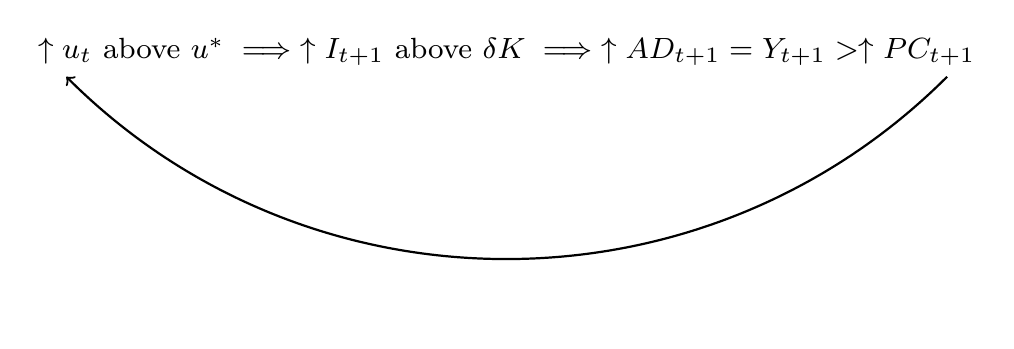
\begin{tikzpicture}{!h}
\node[scale=1.32] at (0,0)(node){$\uparrow u_t \text{ above } u^* \implies \uparrow I_{t+1} \text{ above } \delta K \implies \uparrow AD_{t+1}=Y_{t+1} > \uparrow PC_{t+1}$};
\draw[->, thick]([xshift=-.5cm]node.south east) to [bend left=45]([xshift=.5cm]node.south west);
\end{tikzpicture}
\end{figure}

\paragraph{c)} However, as gross investment increases ($\uparrow I_G$) quarter after quarter so does net investment ($I_N$). The result: $\uparrow PC$ associated with $I=10\text{\euro}$ becomes bigger and bigger.

Ex: when $I_N$ from $90\text{\euro} \implies 100\text{\euro}=\uparrow K \implies \uparrow PC=10\%$

While the $\uparrow AD$ remains the same, 15\euro, (smaller and smaller $\uparrow I$).

Resulting in a smaller and smaller $\uparrow u$ as $\uparrow AD$ becomes closer to $\uparrow PC$. 

\paragraph{d)} Eventually, after many years of expansion, $\uparrow I_N$ to a very high level, from $150\text{\euro} \rightarrow 160 \text{\euro} \implies$


\begin{align*}
\implies \left\{ \begin{array}{r}
    \uparrow PC = 16 \text{\euro} \\ \uparrow AD = 15 \text{\euro}
\end{array} \right\} \implies \downarrow u_t \implies \downarrow I^d_{t+1} \implies \downarrow AD_{t+1} \implies \downarrow Y_{t+1}:\text{ Recession}
\end{align*}

Evidence: 
\begin{itemize}
    \item $\downarrow u_t$ typically between 6 months and 1 year before the end of expansions. 
    \item $\downarrow I$ typically coincides with the end of expansions.
\end{itemize}

\paragraph{e)} 
The recession: $\downarrow u_t$ between 6 months and 1 year before the end of expansions $\implies \downarrow I_{t+1} \implies$ \\ 1 year before the end of the expansion $\implies$
\begin{figure}[H]
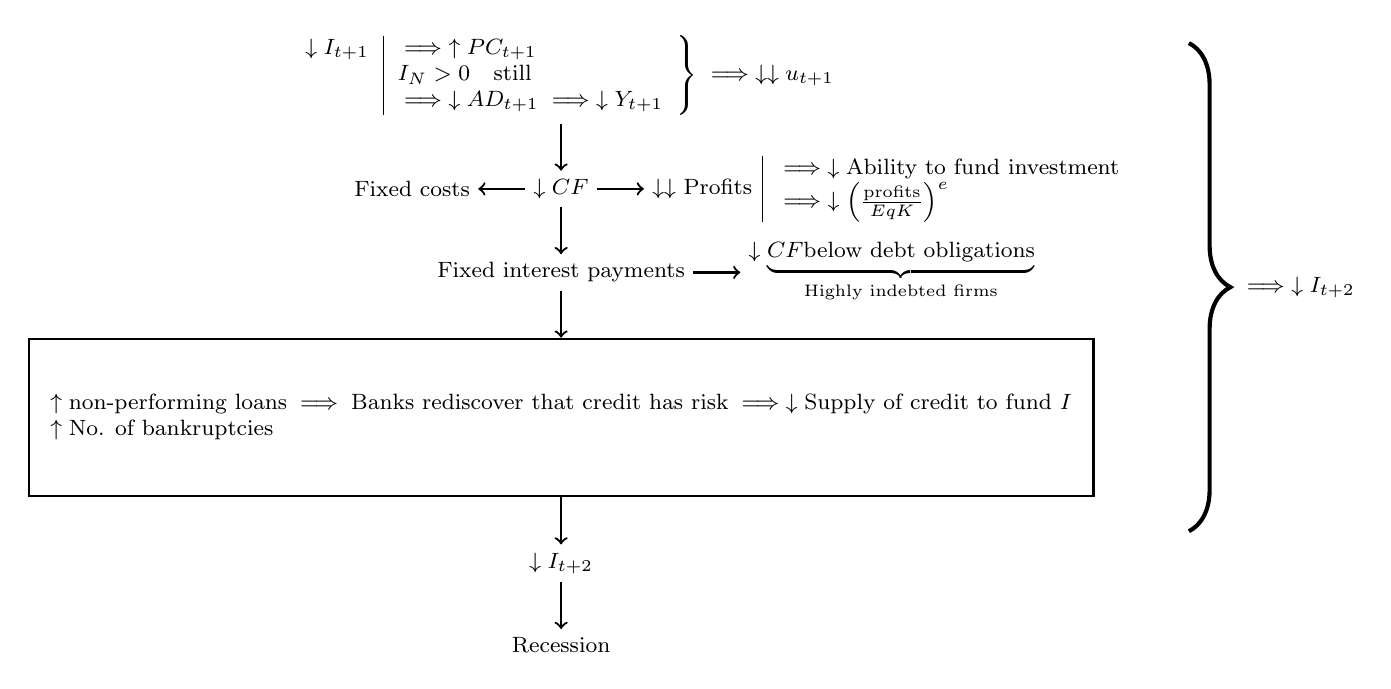
\begin{tikzpicture}[node distance = 2em]
\coordinate (zero) at (0,0);
\node[below = of zero.south west](array){
$\left.\begin{array}{l|l}
\downarrow I_{t+1} & \implies \uparrow PC_{t+1} \\
& I_N > 0 \quad \text{still} \\
& \implies \downarrow AD_{t+1} \implies \downarrow Y_{t+1}
\end{array}\right\} \implies \downarrow \downarrow  u_{t+1}$};
%amplified CF decline
\node[below = of array](cf){$\downarrow CF$};
\node[left = of cf](fc){Fixed costs};
\node[right = of cf](profits){$\downarrow \downarrow$ Profits};

\node[right  = -0.3em of profits]{$\begin{array}{|l}
\implies \downarrow \text{Ability to fund investment} \\
\implies \downarrow \left( \frac{\text{profits}}{EqK} \right)^e
\end{array}$};

\node[below = of cf](interestpayments){Fixed interest payments};
\node[right = of interestpayments](highdebt){$\downarrow \underbrace{ CF \text{below debt obligations}}_{\text{Highly indebted firms}}$};
\node[below = of interestpayments, draw,thick,minimum width=2cm,minimum height=2cm](defaults){$\begin{array}{l}
\uparrow \text{non-performing loans} \implies \text{Banks rediscover that credit has risk} \implies \downarrow \text{Supply of credit to fund } I \\
\uparrow \text{No. of bankruptcies}
\end{array}$};
\node[below = of defaults](it2){$\downarrow I_{t+2}$};
\node[below = of it2](recession){Recession};



%lines
\draw[->, thick] (array) -- (cf);
\draw[->, thick] (cf) -- (fc);
\draw[->, thick] (cf) -- (profits);
\draw[->, thick] (interestpayments) -- (highdebt);
\draw[->, thick](cf) -- (interestpayments);
\draw[->, thick](interestpayments) -- (defaults);
\draw[->, thick](defaults)--(it2);
\draw[->, thick](it2)--(recession);


\coordinate (top) at (8.5,-0.8);
\coordinate (bottom) at (8.5,-7);

%brace
\draw[decorate,decoration={brace,amplitude=15pt, raise = -15pt}, line width=1.5pt] (top) -- node[right, pos = 0.5]{$\implies \downarrow I_{t+2}$} (bottom);



\end{tikzpicture}
\end{figure}


%%%%%%%%%%%%%%%%%%%%%%%%%%%%%%%%%%%%%%%%%%%%%%%%%%%%%%%%%%%%%%%%%%%%%%%%%%%%

\section{The effect of $\uparrow G$ on $\frac{debt}{GDP}$}

\paragraph{a) in a static Keynesian model}

$$\uparrow G^d=1\text{\euro} \implies \uparrow GDP=1.5\text{\euro} \implies \uparrow \text{ tax revenues } + \downarrow \text{ Social transfers}=0.5\text{\euro}$$

Hence, starting from a balanced budget, 

\begin{align*}
\uparrow G=1\text{\euro} \implies \left\{ \begin{array}{r}
     \implies \text{ budget deficit }=\uparrow \text{ Public debt}=1\text{\euro}-0.5\text{\euro}=0.5\text{\euro}  \\
     \implies \uparrow GDP=1.5\text{\euro}
\end{array} \right\} \implies \Delta \frac{debt}{GDP}=?
\end{align*}

\begin{description}
    \item If $\frac{debt}{GDP}=\frac{300\text{\euro}}{300\text{\euro}}$ then $\frac{300.5 \text{\euro}}{301.5 \text{\euro}}<100\%$: $\downarrow \frac{debt}{GDP}$
    \item If $\frac{debt}{GDP}=\frac{100 \text{\euro}}{300 \text{\euro}}=\frac{1}{3}$ then $\frac{100.5 \text{\euro}}{301.5 \text{\euro}}=\frac{1}{3}: \Delta \frac{debt}{GDP}$
\end{description}

Conclusion: 

There will be $\downarrow \frac{debt}{GDP}$ if it's initially bigger than $\frac{1}{3}$ (as it is in almost all countries in the world).

However this is only true in the short term. 

In fact, when the fiscal stimulus is withdrawn: $\downarrow G=1\text{\euro}$, GDP falls back to it's initial value: $\downarrow GDP=1.5\text{\euro}$, to 300\euro. 

But the larger debt remains $\implies \uparrow \frac{debt}{GDP}$ to $\frac{300.5\text{\euro}}{300\text{\euro}}>100\%$. 

\textbf{Conclusion:} except in the short term, $\uparrow G \implies \uparrow \frac{debt}{GDP}$. 

\paragraph{b)} However, 

\begin{figure}[!h]
    \centering
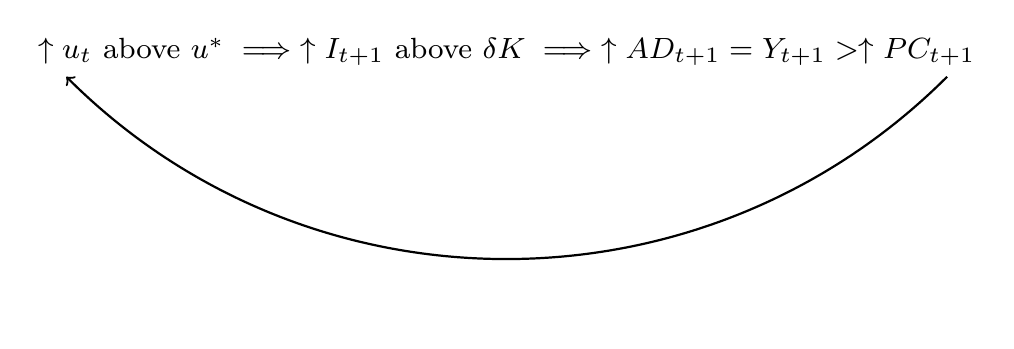
\begin{tikzpicture}{!h}
\node[scale=1.32] at (0,0)(node){$\uparrow u_t \text{ above } u^* \implies \uparrow I_{t+1} \text{ above } \delta K \implies \uparrow AD_{t+1}=Y_{t+1} > \uparrow PC_{t+1}$};
\draw[->, thick]([xshift=-.5cm]node.south east) to [bend left=45]([xshift=.5cm]node.south west);
\end{tikzpicture}
\end{figure}

$$\uparrow GDP$$ year after year, even if $\downarrow G$ back to it's initial level. 

In sum: 

\begin{equation*}
    \uparrow G_t=1\text{\euro} \implies \frac{debt_t}{GDP_t} \text{ from } \frac{300\text{\euro}}{300\text{\euro}} \rightarrow \frac{300.5\text{\euro}}{301.5\text{\euro}}<100\%
\end{equation*}

\begin{description}
    \item In t+1, if $\uparrow I>\downarrow G$, a new $\uparrow GDP \implies \text{ a further } \downarrow \frac{debt \downarrow}{GDP \uparrow}$
\end{description}
Debt will decrease because of the increase of GDP generates bigger tax revenues. 

\paragraph{c)} Illustrative explanation: 


\paragraph{i)} In response to the GR of Jan08-Jun09, there were big $\uparrow G^d$ in the US in Mar09-Dec10 followed by $\downarrow G^d$ in Dec10-Dec13.

\paragraph{ii)} One possible explanation:

$\uparrow G^d$ in March09-Dec10 $\implies \uparrow output$ since July 2009 $\implies u_t$ since July 2009 $\implies$ business I started to increase in Jan10 $\implies \uparrow AD>\downarrow PC \implies \uparrow \uparrow u \implies ... \implies $

\begin{figure}[!h]
    \centering
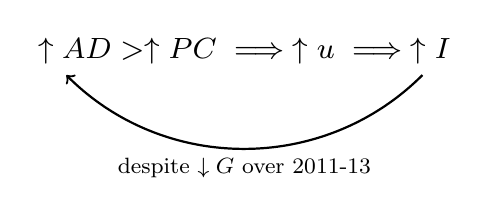
\begin{tikzpicture}{!h}
\node[scale=1.32] at (0,0)(node){$\uparrow AD>\uparrow PC \implies \uparrow u \implies \uparrow I$};
\draw[->, thick]([xshift=-.5cm]node.south east) to [bend left=45]node[pos=0.5,sloped,below]{despite $\downarrow G$ over 2011-13}([xshift=.5cm]node.south west);
\end{tikzpicture}
\end{figure}

\paragraph{iii)} The $\uparrow GDP$ since 2010 $\implies \uparrow \text{fiscal revenue} + \downarrow \text{social transfers} \implies \downarrow \text{ Budget deficit}$ from 10\% GDP in 2009-10 to 2\% GDP in 2015. 

And, $\downarrow \text{ budget deficit} \implies \downarrow \bigg (\uparrow \text{Public Debt} \bigg)$

Two other possible causes for the upper-turning point (besides, $\downarrow u_t \implies \downarrow I^d_{t+1} \implies \downarrow AD_{t+1} \implies \downarrow output_{t+1}$). 

\paragraph{$1^{st}$)} In the last $3^{rd}$ of post 1970s expansions, the prices of $RM+En$ increased by more than the CPI.

$\uparrow \frac{\text{Price of imported }RM+En}{CPI} \implies \downarrow \big[ \big(P-UVC \big)=\text{Unit Profit Margin} \big] \implies \downarrow \text{total profits}$ which further contributed to $\downarrow I_{t+1}^d \implies \downarrow AD_{t+1} \implies output_{t+1}$

\paragraph{$2^{nd}$} After many years of expansion, $\downarrow U$ to very low levels $\implies \uparrow g_{W_N} \implies g_{costs} \implies \uparrow g_P=\uparrow \pi$. This may lead the CB to $\uparrow i_{CB} \implies \downarrow I^d, \downarrow C^d \implies \downarrow AD \implies \downarrow output$.

\section{The Paradox of Thrift}

\paragraph{a)} Static model (Review) $\rightarrow I^d$ fixed by the economic conditions of the previous period. What is the effect of $\uparrow s$ from 20\% to 22\%? 

%%%%%%%%%%%%%%%% grph 

$$\uparrow S \text{ to 22\euro} \implies \downarrow C^d \implies \downarrow AD \implies \downarrow income \implies \downarrow S$$

I spend less $\rightarrow$ you earn less (because my spending is your income) $\implies$ you have less - how much less? 

$$\Delta S= {\color{red}{\uparrow}}s\cdot {\color{red}{\downarrow}} Y$$

Because $S=I$ is fixed in the static model. 

Results: 

$\uparrow S \implies \downarrow C_{today} \implies \downarrow Y_{today} \implies \uparrow U_{today}, \downarrow income_{today} \centernot\implies \uparrow I \text{ and,} \centernot\implies $

$\centernot\implies \uparrow PC\text{ of C goods than otherwise.}$

\paragraph{b)} Dynamic Model 

\begin{figure}[H]
    \centering
    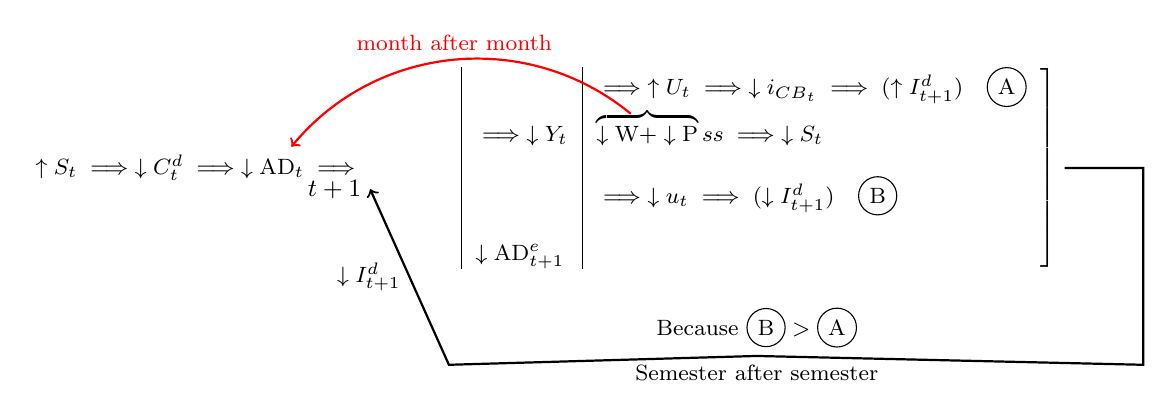
\begin{tikzpicture}
\node (zero) at (0,0){$\uparrow S_t \implies \downarrow C^d_t \implies \downarrow \text{AD}_t \implies$};
\node[right = of zero](array){$ \left. \begin{array}{|l|l}
& \implies \uparrow U_t \implies \downarrow i_{{CB}_t} \implies (\uparrow I_{t+1}^d) \quad \circled{A}
\\ 
 \implies \downarrow Y_t & \overbrace{\downarrow \text{W} + \downarrow \text{P}}{ss} \implies \downarrow S_t \\
\\
& \implies \downarrow u_t  \implies (\downarrow I_{t+1}^d) \quad \circled{B}\\
\\
\downarrow \text{AD}^e_{t+1}
\end{array} \right]$};
\draw[->, thick] (array.east) -- ([xshift=1cm]array.east) -- ([xshift=1cm, yshift=-2.5cm]array.east) -- ([yshift=-1cm]array.south) node[sloped, above]{Because $\circled{B} > \circled{A}$}  node[sloped, below]{Semester after semester} -- ([yshift=-2.5cm]array.west) -- node[left]{$\downarrow I_{t+1}^d$} (zero.south east) node[left]{\small $t +1 $};
\draw[red, thick, ->] ([xshift=-1.6cm, yshift=-0.7cm]array.north) to[bend right = 45] node[pos=0.5, above]{month after month}  ([xshift=-1cm]zero.north east);
\end{tikzpicture}

    \caption{Caption}
    \label{fig:my_label}
\end{figure}


Results:

$\uparrow S \implies \downarrow C_{today} \implies \downarrow Y_{today} \implies \downarrow U_{today}, \downarrow income_{today}$

$$\implies \downarrow I_{tomorrow} \implies \downarrow AD_{tomorrow} \implies \downarrow Y_{tomorrow} \implies \implies \uparrow U_{tomorrow}, \downarrow income_{tomorrow} $$

$$\downarrow I_{tomorrow} \implies \downarrow\text{ Capacity of production of C goods tomorrow (than otherwise)}$$

$$\downarrow AD_{tomorrow} \implies \downarrow Y_{tomorrow} \implies \downarrow u, \text{profits }, \Delta AD_{tomorrow} \implies \downarrow I_{\text{after tomorrow}} \implies$$

$$\implies \left\{ \begin{array}{r}
     \downarrow PC_{\text{ after tomorrow}} \\
     \downarrow AD_{\text{ after tomorrow}}
\end{array} \right\} $$

If we save more we consume less, so firms sell less and produce less, thus, have to lower utilisation and earn fewer profits. So they have reasons to cut investment. 

\section{Paradox of Profits}

$$AD=Y$$

$$C_w^d+\overline{c}^d_p+I^d=W+P$$

$$\overline{c}^d_p+I^d=P$$

\paragraph{a)} Static Model (review) - $\overline{I}^d$ fixed. 

$\downarrow W_N \implies$

$$-\downarrow C^d \implies \downarrow Sales \left\{\begin{array}{r}
   \implies \downarrow Y \implies \downarrow L \implies \downarrow W=w\cdot L\\
   \implies \downarrow P
\end{array} \right\}$$

$$-\uparrow \text{Profits per unit sold}$$

$\implies \Delta Profits=\emptyset$: The paradox of profits, because $Profits=\overline{c}^d_p+\overline{I}^d_{-1}$

\paragraph{b)} Dynamic Model - $I^d(\cdot)$
$\downarrow W_N \implies \downarrow C^d \implies \downarrow Sales$



$$\implies \downarrow Y_t \implies \uparrow U_t \implies \downarrow i_{CB_t} \rightarrow \uparrow (I^d_{t+1})\text{  \circled{A}}$$

$$\implies \downarrow C^d_t \implies \downarrow Sales_t \implies \downarrow Y_t\implies \left\{\begin{array}{r}
\implies\downarrow \text{wage income}_{t}, \downarrow \text{Profit income}_t \\
\implies \downarrow u_t \end{array} \right\}$$
 
 $$  \implies \left\{\begin{array}{r}
     \implies \downarrow S_t  \\
      \implies \downarrow I^d_{t+1} \text{ \circled{B}}
\end{array} \right\}$$

$ - \uparrow \text{Profits per unit sold} $

\section{Minskys explanation of the BC} 

Uncertain Cashflows:
$$CF = P \cdot Q - VC - FC$$

Cash flows consists of all costs except interest costs. Fixed costs include; rents, salaries of overhead workers etc. 

Firms finance their investments in different ways, either through debt or equity capital.
Extremes:
100 \% debt financed or most funding by equity capital. 


Fixed payments that are imposed by debt
\begin{itemize}
    \item Interest payment
    \item Debt payment (amortizations)
\end{itemize}

\paragraph{ROA = Return of Assets}  Tells us how profitable machines are. $\frac{CF}{A} = 9\%$ In this example the machine gives 9 cents in return.

\paragraph{ROE = Return of Equity}  

$$\frac{CF - \text{Interest payments}}{E_f} = 10 \%$$

In this example, shareholders get 10 cents for each stock they own. 

In a company without debt ROA = ROE.

\subsection{Explain the variance of phases of the BC}

\subsubsection{How a recession leads to a depression}

A depression is a stagnation at a low level following a recession
\paragraph{a)} The recession:
$$\downarrow AD \underset{\text{fixed costs}}{\implies} \text{amplified} \downarrow CF \implies \text{CF of many firms fall below their debt commitment} \implies \text{Defaults}$$

$$ \implies \left\{\begin{array}{r}
     \text{Losses for banks}  \\
     \text{Many bankruptcies} 
\end{array} \right\}$$



Cash flows fall in an amplified manner following a decline in sales. Many defaults on loans, leads to losses for banks. Many firms go bankrupt because they are unable to meet their debt commitments. 

Cash flows become insufficient to cover debt obligations. This negative experience of firms and banks explains the depressions following a recession.

\paragraph{b)}  The memories of this make banks only want to loan to firms with low debt compared to assets $\frac{\text{debt}}{A} = \frac{10}{100}$

The firms with low debt commitments have small fixed payments on  debts, 10 \% of 10 = 1, and uncertain cashflows derived from large assets.. This implies a low probability of default.  
\begin{itemize}
    \item Banks are cutting down on credit. 
    \item Firms are less willing to take loans and the debt ratio is decreasing.
\end{itemize}

Firms also want low debt ratios. 

\paragraph{c)} Consequence:
Firms ask for very few loans to fund new investment. 

Banks become very selective in granting loans for new investment. Low and not $\uparrow I \implies \text{low and not} \uparrow AD, \uparrow Y$: Stagnation. 

\subsubsection{3. a) As time goes on with firms with low $\frac{debt}{A}$}

How low can ROA fall, while maintainaing a cashflow high enough to cover interest payments? The ROA may fall as low as 1\% and $CF=1\%100\text{\euro}\geq10\text{\euro}$ which is equal to it's debt commitments $=10\%10\text{\euro}$. 
If the firm is highly in debt:

$$\frac{\text{Debt}}{A} = \frac{100}{100}$$

CF = 100 
Debt commitment = 1 (small) 10 \% 10

For $\frac{1\%}{ROA} CF \geq debt$

R.O.A must be greater than 10\% for CF 10\% of 100 > debt payments

With low debt, the debt payment is smaller and a lower cash flow can be tolerated.

Banks and firms remember the recent recession and are more cautios. Leading to a lower AD, because the demand for capital goods is low. Low and not rising AD and output $\rightarrow$ Stagnation

The stagnation that follows a recession is explained by fear in banks and firms. 

\paragraph{b)} As time goes by with firms with low debt ratios. 

Firms can easily meet their debt payments. 

The memories of the non-performering loans fade. Confidence grows, fear gradually subsides. 

Banks and firms start accepting higher debt ratios. 

\paragraph{c)} Moreover, as long as ROA $\geq$ interest rate 

Firms can increase profits and profits rates if they undertake new I projects funded with debt:

\begin{figure}[!h]
    \centering
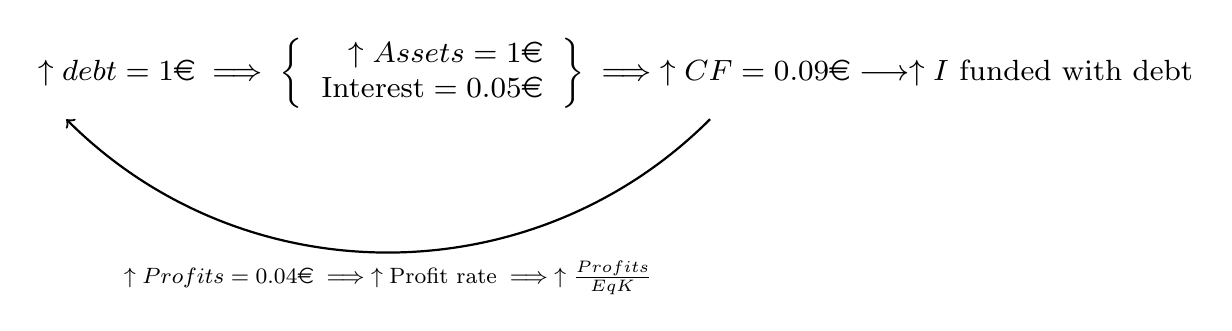
\begin{tikzpicture}
\node[scale=1.32] at (0,0)(node){$\uparrow debt=1\text{\euro} \implies \left\{\begin{array}{r}
      \uparrow Assets=1\text{\euro} \\
      \text{Interest}=0.05\text{\euro}
\end{array} \right\} \implies \uparrow CF=0.09\text{\euro} \longrightarrow \uparrow I \text{ funded with debt}$};
\draw[->, thick]([xshift=1.2cm]node.south) to [bend left=45]node[pos=0.5,sloped,below]{$\uparrow Profits=0.04\text{\euro} \implies \uparrow \text{Profit rate} \implies \uparrow \frac{Profits}{EqK}$}
([xshift=.5cm]node.south west);
\end{tikzpicture}
\end{figure}

Debt of 1, interest payment of 5 cents, with this loan the firms buys a machine for 1 euro which gives 9 cents. Profits rise by 4 cents. Profit rate goes up because the equity capital stays the same, but profits has increased by 4 cents. 

Shareholders have not invested more in equity capital, as the new investment was financed with debt. 

\subsubsection{4. Expansion:}

Firms want to increase investment funded by an increasing share of debt to profit from the financial leverage. Buying more machines with loans, the higher is the profit increase while their equity stays constant. The more profit rates rise. Banks are willing to extend the corresponding loans. 

Firms want to increase investment funded on increasing share of debt, and banks are willing to extend the corresponding loans. 

\begin{figure}[!h]
    \centering
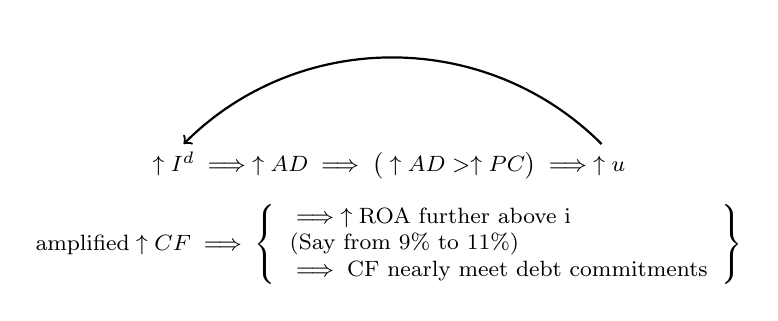
\begin{tikzpicture}
\node[scale=1] at (0,0)(zero){$\uparrow I^d \implies \uparrow AD \implies \big(\uparrow AD> \uparrow PC \big) \implies \uparrow u$};
\node[scale=1] at (0,-1)(one){$\text{amplified} \uparrow CF \implies \left\{\begin{array}{l}
     \implies \uparrow \text{ROA further above i}  \\
     \text{(Say from 9\% to 11\%)} \\
     \implies \text{CF nearly meet debt commitments}
\end{array} \right\}$};
\draw[->, thick]([xshift=2.7cm]zero.north) to [bend right=45] ([xshift=.5cm]zero.north west);
\end{tikzpicture}
\end{figure}

Magic of deleveraging. 

Sometimes doesn’t happen in real world, however, Minsky says that relative to gdp and to assets, debt increases during the expansion (shadow period) then right afterwards it should fall, because both banks and firms have bad memories of defaults in previous recessions, thus debt should fall in the first years of the expansion, and then as the bad memories fade, debt starts to rise again. 

\subsection{The explanation for the beginning of recessions}

\paragraph{a)} After many years of funding, investment with an increasing proportion of $\frac{\text{Debt}}{\text{Assets}}$, firms have high debts relative to their assets. $\implies$ high fixed debt payments $\implies$ amortisations and interest payments.

The debt is high compared with their uncertain cash flow. Cash flows are uncertain because sales are uncertain.

Both of these aspects makes firms vulnerable to two sort of effects:

\paragraph{1)} They are vulnerable to increases in $i_{CB}$ (Central bank may raise interest rates after many years of expansion due to low unemployment  the natural rate, which makes workers bargaining power stronger where they can demand an increase in the rate of growth of their nominal wages)
To fight inflation $\Pi$ and low unemployment.

Rising debt obligations above CF increases loan defaults for indebted firms

According to Minsky the beginning of recession comes because of an increase in defaults, because of an increase in the interest rate of CB which raises debt obligations above CF

CF = Revenue - Variable Costs - Fixed Costs (except interests)

\paragraph{2)} $\downarrow u$ Towards the end of expansion the rate of utilisation drops, typically 1 year before the onset of the recession. After a while $$\downarrow I^d \implies \downarrow AD \implies \downarrow \text{Sales}$$

Investment goes down, the demand for machines and office buildings goes down. AD goes down and then sales goes down, however, firms still have fixed costs $\rightarrow$ CF falls in an amplified manner.

For some firms CF may fall below debt commitments  and this increases the number of defaults. 

The reduction in cash flow can come from both a reduction in sales and an increase in $i_{CB}$

The increase in defaults can be very restricted, for instance only in firms with high debt or firms very sensitive to demand fluctuations. 

\paragraph{b)}

Because what banks consider acceptable debts/assets ratios is highly subjective, but once they observe some defaults somewhere in the economy, they may suddenly make drastic downward revisions in what deem to be acceptable ratios. 

This moment of «awakening» is called the \textbf{Minsky Moment}, it is the moment when after a long period of complacency towards credit, banks suddenly rediscover that credit implies the risk of default. -> Banks panic, too much debt. Cut the debt ratio down. Banks make wide cuts in the supply of credits to firms. 

With a lower access to credit, investment goes down, and so does consumption and AD because of the multiplier.

Rate of utilisation goes down, profits goes down, leading to a further decline in investment. 

Amplified reduction in CF with the consequence increasing the number of defaults. Amplifying the recessive spiral and tightening the supply of credit to firms and banks are afraid of credit in general (households not initally but after a while). Consumption that is typically financed with debt (cars etc) wil also suffer. The increase in defaults leads to losses for banks as well. 

The above is Minskys explanation of a recession: «Credit Crunch»: banks tightening the supply of Credit.

\paragraph{} What happens to the the ratio of debt/GDP in recessions?

Debt should go down because banks cut credit access. Banks cut credit to BH. The absolute value of debt in the economy should decrease during recessions. 

They reduce new loans, i.e. Harder to get new loans and they reduce the renewals of old loans. 

The fact that firms spend income to pay down their debt, will push down GDP. If the decline in GDP is bigger than the decline in debt, the ratio will increase. This money would've, otherwise, been spent on goods and services, and thus AD falls. 

What do firms do when they are faced with declining sales? They cut output. 

Before WWII, when faced with falling sales, firms cut both prices and incomes. The debt to GDP ratio may rise if the denominator ends up falling by more than the numerator.

In the great recession prices fell by 25\% and GDP fell by 30\% and debt increased 20\% and the ratio.

In other prewar recessions, something similar happened. 

What about post war recessions?
Sometimes they rise a little, but debt is falling, the decline in debt is causing the decline in demand. The essential reason:
As firms and household are forced to pay down debt, they don’t use the money for goods and services. 

\subsection{The paradox of deleveraging}
\paragraph{Paul Krugman:} My Spending is your income, and your spending is the income of my firm. When we are both forced to cut spending in order to pay our debts, this reduces our incomes - in such a way that even though our debts diminish, they rise relatively to our incomes.

In a recession we are both forced by banks to cut spending, this reduces our incomes. When I cut my spending your income falls, vice versa. 

This may happen in such a way that even though our debts go down, they rise relative to our incomes.
At the end of the expansions firms debt is quite high relative to their assets. 

90\% of their machines are financed with debt, only 10\% with equity capital. Firms have high fixed debt obligations to their uncertain cashflows. 

\subsection{The Sub-Prime credit crisis of 2007-8 which lead to the great recession of 2008-2009}

Minsky said that recessions are triggered by an increase in defaults somewhere in the economy. 

The same idea can be presented for the case of households defaulting on their debts, that is the main explanation of the world recession of 2008-2009.

The explanation:

\paragraph{a)} From 2002 until 2006, in the US, there was a big increase in credit granted to the purchase of houses. This big increase in credit involved 2 features:
\begin{enumerate}
    \item Variable interest rates/indexed rates. 
    \item Implied big monthly instalments compared with peoples monthly wages. 
\end{enumerate}
\paragraph{b)} Beginning in 2005 the Fed started to raise interest rates from the low level of 2\% all the way up to 5.25\% in July 2006. This lead to a big increase in the monthly payments on house credit for households who had previously contracted credit with variable rates. Beginning in Jan 2007 the number of defaults on mortgage credits increased, especially on sub-prime (variable rates) credit. 

\textbf{Banks rediscover credit risk - minsky moment}

Wide cuts in credit supply $\rightarrow$ AD down $\rightarrow$ GR08-09

Minsky provided a good explanation of the GR

Big increase in Variable Sub Prime loans, which made up about 7\% of total mortgage credits, but by the middle of the year of 2007 they had almost half of all defaults in the US. 


\subsection{The Eurozone sovereign debt crisis of 2010-2013}

\begin{enumerate}
    \item  The Great Recession lead to decreases in tax revenue and increase in public expenditure, unemployment benefits and household (discretionary expenditures in 2009 and 10). Private AD was declining and governments attempted to counter it with raising public expenditure. With the consequence of skyrocketing budget deficits to roughly 10\% of GDP in many 1st world countries.
    
    The consequences of this was a big increase in public debt relative to GDP. 
    
    \item In December 2009 the EC discovered that the Greek government had falsified heir accounts. The deficit numbers were fake and they suspected Greece would be unable to repay its debt. In May 2010 the German and French banks started to suspect that other sovereign governments, because of the their high debt ratios would also be unable to repay their debts. Leading to Austerity programmes $\implies$ deep recessions in the south of Europe, big increases in unemployment. 

Sharp decline in supply of credits to those governments  which as a result were forced to make big cuts in their budget deficits $\implies$ Leading to austerity $\implies$ Cut in Public spending and increase taxes as well as a cut of transfer to the private sector, and cut in unemployment benefits and public pensions. A decline in disposable income leading to a decline in consumption leading to $\downarrow AD$ increased unemployment etc.
\end{enumerate}

\chapter{Currency crises in fixed exchange rates}

\section{Basic notion of open economy macro}

\subsection{Domestic and total demand}

\begin{equation*}
\begin{array}{lcl}
AD = 100 & \implies & \text{Output} = 100 \\
& \implies & \text{Total revenues of firms 100, which they entirely use to pay the factors of production (wages,rents, interest and profits), hence} \\ & \implies & AD \equiv \text{\sc Output} \equiv \text{\sc Income} \end{array}
\end{equation*}

\subsection{}
\begin{equation*}
\begin{array}{lcl}
D_{\text{Total}} & = & D_{\text{Total}} - M^d + X^d  \\
AD & = & DD - M^d - X^d \\ &  & C^d + I^d + G^d \end{array}
\end{equation*}
	
	\subsection{Trade Balance}
	
	$$TB=\text{Output} - DD = X - M$$
	
	China 2000 - 10
	
	Trade balance stuff
	
	\subsection{A country is comprised of two sectors}
	
	
\begin{equation*}
\begin{array}{lcl}
TB & = & \text{Income} - DD  \\
TB & = & (\text{Government income} - G^d) + (\text{Private sector Income} - C^d - I^d) \\
TB & = & \underbrace{(T - G)}_{\text{\sc Public Balance}} + \underbrace{(S - I)}_{\text{\sc Private Balance}} \end{array}
\end{equation*}

\begin{equation*}
\begin{array}{lll}
-10 = -3 - 7  & \}  & \text{Portugal 1999-08} \\
-10 = -10 + 0  & \} & \text{Portugal 2009-10}
\end{array} \Biggr\}
\text{Deficit = 10\% of GDP}
\end{equation*}

In sum: 
\begin{enumerate}
    \item $\text{AD} \equiv \text{\sc Output} \equiv \text{\sc Income}$
\item $\text{AD} = \text{DD} - M^d + X^d $
\end{enumerate}



\section{The effect of a trade imbalance on M1(C + CD), M2(C + CD + SD)}

Argentina 
$$\text{TD} = 1P \implies \text{DD} = \text{Output (=Income)} + 1P$$ 
How can the Argentinian residents finance the difference?

\subsection{From past savings}
\begin{figure}[H]
    \centering
       \tikzset{redline/.style={draw, red, line width=1pt, ->, shorten >=5pt, shorten <=5pt}}


\begin{tikzpicture}[node distance = 100pt]
\node(center){M firms  = 2\$};
\node[below = of center](RW){RW};
\node[above = of center](residents){Residents};
\node[left = of center](X){X= 1};
\node[right = of center](banks){Banks};
\node[right = of banks](CB){CB};

%Horizontal
\draw[redline] (center.south west) to [bend left=45] node[pos=0.5,sloped,below]{1P}(X.south east);
\draw[redline] (X.north east) to [bend left=45] node[pos=0.5,sloped,above]{1\$} (center.north west);

\draw[redline] (banks.north west) to [bend right=45] node[pos=0.5,above]{1\$} (center.north east);
\draw[redline] (center.south east) to [bend right=45] node[pos=0.5,below, align=right]{$ \begin{array}{c} \underbrace{CD = 1P}_{\text{\sc Money is destroyed}} \\  \downarrow CD = 1P \end{array}$} (banks.south west);

\draw[redline] (CB.north west) to [bend right=45] node[pos=0.5,above]{1\$} (banks.north east);
\draw[redline] (banks.south east) to [bend right=45] node[pos=0.5,below]{R = 1P} (CB.south west);


%Vertical Lines
\draw[redline] (center.south) to [bend left=45] node[pos=0.5,right]{2\$} (RW.north east);
\draw[redline] (RW.north west) to [bend left=45] node[pos=0.5,left]{Goods} (center.south);

\draw[redline] (center.north) to [bend left=45] node[pos=0.7,left]{Goods} (residents.south west);
\draw[redline] (residents.south east) to [bend left=45] node[pos=0.3,right]{$CD = 1P \leftarrow SD = 1 ; \uparrow CD = 1P, \downarrow SD = 1P$} (center.north);


\end{tikzpicture}
    \caption{Financing a trade deficit with past savings}
\end{figure}

In fixed rates the CB is obliged to this (exchange rates) to prevent a depreciation of Peso. 

CD In peso remain the unchanged, first ... and then decrease

\subsubsection{Overall Results}

\begin{equation*}
\begin{array}{lllll}
\downarrow SD & = & 1P = TD & \implies & \downarrow M2  \\
\Delta CD & = & +1P -1P = \emptyset & \implies & \Delta M  \\
\Delta M1 & = & \emptyset = \& & \implies & \Delta M2 = -1  \\
\text{CB}_{\text{Reserve}} & = & 1\$ & = & TD  \\
\text{R}_{\text{Pesos}} & = & 1P & = & \downarrow MB  

\end{array}
\end{equation*}

IBMM:
$$
\underset{\text{\sc Excess R}}{\text{Banks}} \underset{\text{\sc Loans}}{\rightarrow} \underset{\text{\sc Lack of R}}{\text{Banks}}
$$

Excess domestic reserves in the IBMM = 1p = tendency for $\uparrow i_{IBMM}$ to prevent this, the CB is forced to inject R = 1p how? Through open market purchases of treasury bills: 

\begin{figure}[H]
    \centering
       \tikzset{redline/.style={draw, red, line width=1pt, ->, shorten >=5pt, shorten <=5pt}}

       \tikzset{blueline/.style={draw, blue, line width=1pt, ->, shorten >=5pt, shorten <=5pt}}

\begin{tikzpicture}[node distance = 10em]
\node (TD) {TD};
\node[right = of TD](banks){Banks};
\node[right = of banks](cb){CB};

\draw[redline, very thick] (TD) -- (banks);
\draw[redline] (banks.south east) to [bend right=45] node[pos=0.5,sloped,below]{R =1P}(cb.south west);
\draw[redline] (cb.north west) to [bend right=45] node[pos=0.5,sloped,above]{1\$}(banks.north east);

\draw[blueline] (banks.north) to [bend left=105] node[pos=0.5,sloped,above]{TB's=1P}(cb.north);
\draw[blueline] (cb.south) to [bend left=105] node[pos=0.5,sloped,below]{1P}(banks.south);



\end{tikzpicture}
    \caption{Sterilisation}
\end{figure}

$$\Delta i_{\text{IBMM}} = \emptyset$$

The $\downarrow R$ caused by TD is sterilised by firms

\subsection{Loans from domestic banks}

\begin{figure}[H]
    \centering
    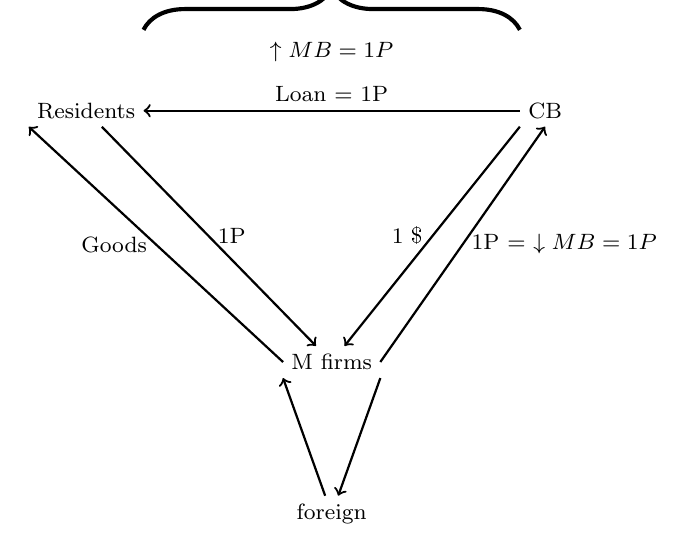
\begin{tikzpicture}[node distance = 8em]
\coordinate (zero) at (0,0);
\node[left = of zero](residents){Residents};
\node[right = of zero](cb){CB};
\node[below = 10em of zero](firms){M firms};
\node[below = 5em of firms](foreign){foreign};



\draw[->, thick] (cb)-- node[above, pos=0.5]{Loan = 1P}(residents);
\draw[->, thick] (cb.south west)-- node[left, pos=0.5]{1 \$}(firms);
\draw[->, thick] (firms.east)-- node[right, pos=0.5]{1P = $\downarrow MB= 1P$}(cb.south);
\draw[->, thick] (residents)-- node[right, pos=0.5]{1P}(firms);
\draw[->, thick] (firms.west)-- node[left, pos=0.5]{Goods}(residents.south west);
\draw[->, thick] (firms.south east) -- (foreign);
\draw[->, thick] (foreign) -- (firms.south west);
\draw[decorate,decoration={brace,amplitude=15pt, raise = 15pt}, line width=1.5pt, transform canvas={yshift=0.5cm}] (residents) -- node[above, pos = 0.5]{$\uparrow MB = 1P$} (cb);
\end{tikzpicture}
    \caption{Financing a trade deficit with domestic loans}
\end{figure}

$$TD = 1P \implies DD = \text{Income} = 1P$$

This 1P is obtained through loans form domestic banks, to simplify from CB.
$$TB = X - M \implies -1 \$ = 0 - 1 \$ $$
\paragraph{Results:}
\begin{description}
    \item $\downarrow \text{CB's Reserves}=1\$=TD$ (previous case)
    \item $\uparrow MB=1P \text{ followed by} \downarrow MB \implies \Delta MB=\emptyset$
\end{description}

\subsection{Loans from foreign banks}

\begin{figure}[H]
    \centering
    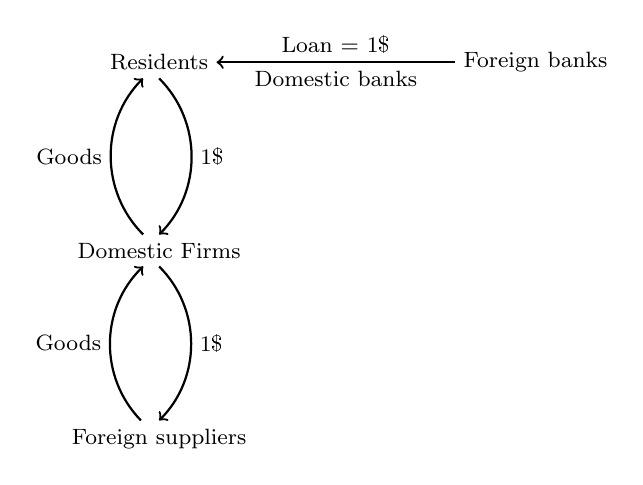
\begin{tikzpicture}[node distance = 8 em]
\coordinate (zero) at (0,0);
\node[right of = zero](foreign_banks){Foreign banks};
\node[left of = zero](residents){Residents};
\node[below of = residents](firms){Domestic Firms};
\node[below of = firms](foreign_suppliers){Foreign suppliers};

\draw[->, thick](foreign_banks) -- node[above, pos=0.5]{Loan = 1\$} node[below, pos=0.5]{Domestic banks} (residents);

\draw[->, thick](residents.south)to [bend left = 45] node[right, pos=0.5]{1\$}(firms.north);
\draw[->, thick](firms)to [bend left = 45] node[left, pos=0.5]{Goods}(residents);


\draw[->, thick](firms.south)to [bend left = 45] node[right, pos=0.5]{1\$}(foreign_suppliers.north);
\draw[->, thick](foreign_suppliers)to [bend left = 45] node[left, pos=0.5]{Goods}(firms);

\end{tikzpicture}
    \caption{Financing a trade deficit with foreign loans}
\end{figure}


\paragraph{Results:}
\begin{enumerate}
    \item $TD=1\$=\uparrow\text{external debt }=1\$$ instead of the changes in Reserves or savings deposits of the other two cases;
    \item Any exchange in bank's Peso Reserves? No, thus $\Delta i_{IBMM}=\emptyset$;
    \item $M_1$ and $M_2$ are unchanged as well.
\end{enumerate}

\section{Institutional International Financial Investors (IFI)}

\begin{figure}[H]
    \centering
           \tikzset{redline/.style={draw, red, line width=1pt, ->, shorten >=5pt, shorten <=5pt}}

       \tikzset{blueline/.style={draw, blue, line width=1pt, ->, shorten >=5pt, shorten <=5pt}}
        \begin{tikzpicture}[node distance = 6em]
        \draw (0,0) circle (4);
               \draw  (3*0.866,-3*1.01) -- (0,0) -- (-3*0.866,3*1.01);
                \draw  (3*0.866,3*1.01) -- (0,0) -- (-3*0.866,-3*1.01);
                \coordinate (center) at (0,0);
                \node[left = of center]{Bonds GM};
                 \node[right = of center](GM){$TB_A$};
		 \node[below = 6em of center]{$TB_{US}$};
		\node[above = 6em of center]{Stocks BP};
		
		\coordinate (north_east_bound) at (3*0.866,3*1.01);
		\coordinate (south_east_bound) at (3*0.866,-3*1.01);
		\coordinate (south_west_bound) at (-3*0.866,-3*1.01);
		\coordinate (north_west_bound) at (-3*0.866,3*1.01);




	\node[above = 20 em of center, align=left](private_ss){SS contributions of workers, \\ automatically deducted form their paychecks.};
	\node[below right = of private_ss, align=left](public_ss){Public SS. \\ PPFS (UK and US)};
	\node[right = 2em of GM, align=left](portfolio){Diversified portfolios of \\ stocks and bonds in different \\ countries/markets.};
	\node[below left = 10em and -3em of portfolio](insurance){Insurance companies};
	\node[right = of insurance](pp1){People};
	\node[below left = 6em of south_west_bound, align = left](PPFS){PPFS \\ Mutual funds \\ Hedge Funds};
	\node[right = of PPFS](pp2){People};
	
	\node[above left = 6em of north_west_bound](banks){Investment banks};
	\node[above = of banks](commercial_banks){Commercial banks};


	



	\draw[redline](private_ss.south east) -- node[pos=0.5, sloped, above]{P} (public_ss);
	\draw[redline](public_ss.south west) -- node[pos=0.5, right, sloped, above]{P, \$, \text{\euro}} (north_east_bound);
	\draw[redline](insurance) -- node[pos=0.5, right, sloped, above]{P, \$, \text{\euro}} (south_east_bound);
	
	\draw[redline](PPFS) -- node[pos=0.5, sloped, above]{P, \$, \text{\euro}} (south_west_bound);
	\draw[redline](banks) -- node[pos=0.5, sloped, above]{P, \$, \text{\euro}} (north_west_bound);
	
	\draw[redline] (commercial_banks) -- node[pos=0.5, right]{\text{Loans} = P} (banks);

	\draw[redline] (pp1.south) to [bend left=45] node[pos=0.5,sloped,below]{\text{Insurance Policies}} (insurance.south);
	\draw[redline] (insurance.north) to [bend left=45] node[pos=0.5,sloped,above]{P}(pp1.north);
	
	\draw[redline] (pp2.south west) to [bend left=45] node[pos=0.5,sloped,below]{P}  (PPFS.south east);
	\draw[redline] (PPFS.north east) to [bend left=45] node[pos=0.5,sloped,above]{Shares}(pp2.north west);




    \end{tikzpicture}
    \caption{Caption}
\end{figure}

If for some reason IFI start expecting that the P will depreciate:
COMMENTED
% $\implies$ they sell a significant part of their P securities. Exchange the Pesos they obtained for \$ with Argentina's CB $\implies $\downarrow \text{ Reserves}$ , eventually to $\emptyset \implies $ IFI will have Pesos to exchange and no one to exchange them with $\implies$ depreciation.

Self-fullfiling Prophecy:Expectation that the Peso will depreciate in the future $\implies$ depreciation of the Peso in the present. 

%Investors/Speculators suddenly start believing that a string of past succesive trade deficits caused by a string past succesive budget deficits will continue in the future. TDs (<- BDs) Eventually deplete the \$ reserves of the central bank. They flee out of the country currency. Investors hold secuirities in the currency that is depreciating. They sell securities to obtain the currency, then exchange it for \$. 

%Speculators short sell the currency, and deplete the CB reserves. 

%Afterwards we get a depreciation in the currency. 

%Investors avoid losses by selling securities, speculators profit by short selling. 

\section{First generation explanation for currency crises} 

$$AD = C^d(Y,i) + I^d(u_{t-1}, P_{t-1}, \Delta AD_{t-1}, i_{t-1}) + G^d - M^d(Y) + X^d(Y_{??})$$

\begin{equation*} \text{Start from}
    \left\{\begin{array}{l}
    \text{Full employment}   \\
     TB = \emptyset = BB + BP
    \end{array}\right. \implies E_0
\end{equation*}



\begin{figure}[H]
\centering
\begin{subfigure}{.5\textwidth}
  \centering
 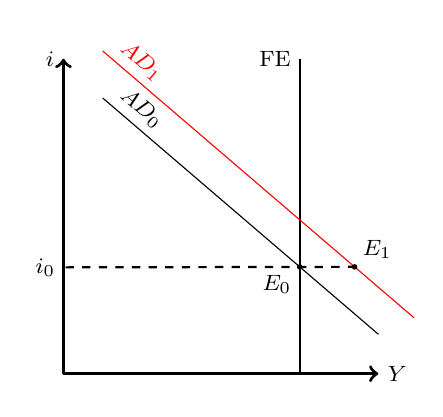
\begin{tikzpicture}
%First Graph
\coordinate (zero) at (0,0);
\draw[very thick, ->] (zero) -- (4,0) node[right]{$Y$};
\draw[very thick, ->] (zero) --  (0,4) node[left]{$i$};



\draw[name path = FE,thick] (3,0) -- (3,4) node[left]{FE};

\draw[name path = AD0] (0.5,3.5) -- node [pos = 0.1, sloped, above] {$AD_0$} (4,0.5);
\draw[name path = AD1, yshift= 2em, shorten >= -2em, red] (0.5,3.5) -- node [pos = 0.1, sloped, above] {$AD_1$} (4,0.5);



\coordinate[name intersections={of=AD0 and FE,by=E0}];
\node[left] at (0,1.35)(i0){$i_0$};


\draw[name path= i0, dashed, thick] ([xshift=2.4em]E0) -- (i0);
\node[below left] at(E0){\footnotesize $E_0$};
\fill[black] (E0) circle (1pt);


\coordinate[name intersections={of=AD1 and i0,by=E1}];


\node[above right] at (E1){\footnotesize $E_1$};
\fill[black] (E1) circle (1pt);
\end{tikzpicture}
  \caption{A subfigure}
  \label{fig:sub1}
\end{subfigure}%
\begin{subfigure}{.5\textwidth}
  \centering
\begin{tikzpicture}[decoration={triangles}]

%second Graph
\coordinate (zero) at (0,0);
\draw[very thick, ->] (zero) -- (4,0) node[right]{$Y$};
\draw[very thick, ->] (zero) --  (0,4) node[left]{$TB$};
\draw[very thick, ->] (zero) --  (0,-2);


\draw[thick] (3,0) -- (3,4) node[left]{FE};
\coordinate (e0) at (3,0);
\coordinate (e1) at (3.8,-0.6);




\node[above right]  at (e0) {$E_0$};
\node[below right] at (e1) {$E_1$};




\draw[postaction={draw,decorate}, red](e0) -- (e1);
%\draw[postaction={draw,decorate}, red](e1) -- (e2);




\fill[black] (e0) circle (1pt);
\fill[red] (e1) circle (1pt);




\end{tikzpicture}
  \caption{AD}
  \label{fig:sub2}
\end{subfigure}
\caption{Graphs showing effects of external \textbf{positive} shocks in fixed exchange rate regimes}
\label{fig:test}
\end{figure}

For some reason the Government starts applying an expansionary monetary policy:

\begin{equation*} \uparrow G^d \implies
    \begin{array}{|l}
     \implies \uparrow AD \implies \uparrow Y_{> FE} \implies \uparrow \Pi \\
     \implies  \uparrow M \implies TD
    \end{array}
\end{equation*}

The increase in public spendings will be funded in two ways:

\begin{enumerate}
    \item Emission of treasuby bills in USD bought by IFI/ \$ loans from foreign banks:
    \begin{description}
        \item $\uparrow$ External debt
        \item The gov pays for M with the borrowed \$, not with \$ Reserves of the CB
    \end{description}
 \item Emission of Treasury bills in P in the domestic primary market/ P Loans from domestic banks:
 \begin{description}
     \item The government exchanges Pesos for \$ with the CB to buy imports M $\implies \downarrow \text{CB's \$ Reserves}$.
 \end{description}
\end{enumerate}

The gov exchanges ... for USD with the CB to .. M $\implies \downarrow \text{Reserves}_{\$} $

\paragraph{After a few years of Trade deficit}
\begin{enumerate}
    \item Foreign banks and IFI will start suspecting that the government will eventually be unable to repay it's debt $\implies$ stop extending new loans $\implies$ the governemnt will have to turn to the other source of funding (domestic) only.
    \item IFI will start expecting that the declining path of the central banks dollar reserves is irreversible and will become stepper.
\end{enumerate}

They predict, at a period $t_c$, that the central bank will run out of reserves at $t_d$, and they will plan a flight out of the Peso at $t_{d-1}$. But if all IFI think like this, \$ reserves will be depleted at $t_{d-1}$, so they will plan the flight for $t_{d-2}$, and this line of reasoning will lead IFI to flight at $t_c$.


\subsection{Conclusion}
\begin{enumerate}
    \item The currency crises results from an incompatibility between the position of the economy and the fixed rates
    \item The fixed rates end well before the central banks' dollar reserves are depleted
    \item The moment when fixed rates end is independent of the amount of dollar reserves initially owned by the CB: 
    \begin{itemize}
        \item If the amount had been large, moment $t_d$ would have been further to the right, but the currency crisis would occur at $t_c$:
        The moment when IFI + speculators realise that the trade deficit will inevitably deplete the reserves. 
    \end{itemize}
\end{enumerate}

\subsection{Summary}
\begin{enumerate}
    \item Investors and speculators believe that a a string of past succesive trade deficits (caused by budget deficits) is to continue in the future eventually deplete the reserves of the central bank.
    \item They flee out of the currency leads to quicker depletion of the reserves. followed by depreciation. 
    \item Speculators make profits while investors avoid losses. 
\end{enumerate}

\section{2nd generation explanation for currency crises} 

There is no risk whatsoever of depletion of CB reserves. What causes the flight of investors and speculators?

Leaving fixed rates and let the currency depreciate implies both  BENEFITS and COSTS for the country’s economy. 

When speculators suspect that the benefits of leaving have become bigger than the costs. They suspect the government will let the currency depreciate, as a result they will run away from the currency. 

\subsection{3 historical examples:}
\paragraph{Argentina in 1999-2000}
-> 1P = 1\$ -> towards the end of 90s, there was an apreciation of the dollar and as a result the Argentoine peso also appreciate. 1P = 1 BRL -> 2 BRL

Consequence, the price of exports from Arg to BR went up. 

Exports from Argentina became expensive in Brazil, and exports went down. 

Imports from Brazil became cheaper in Argentina and imports went up.

\paragraph{France May 1968}
Student revolution + countrywide strikes. 
Consuqence: Large increases in nominal wages, implication, big increases in Unit Production Costs in France. Emphasize the costs of 2 secotrs:\
French exports: 
French Companies that competed with imports:

Decline in exports, and increase in imports. 

\paragraph{In 1982-1992 Spain/Italy}
$$\Pi_{\text{IT, ESP}} = \Pi_{\text{GER, FR}} + 3pp.$$

Prices in Italy and Spain increased 30\% more than in France and Germany. Nominal wages increased by 30\% more than in France and Germany \
Conseuqnce: 
$$\begin{array}{l|l}X^d \downarrow M^d  \uparrow = \end{array} \quad \text{Loss of competitivness}$$

\subsubsection*{QUESTION: Which may be the benefits and costs of leaving fixed rates}

1. Adjustment problem
Start from $FE and TB = BB + PB = \emptyset$

Assume both public and private are spending as much as they earn = balance. Thus, the trade balace is in eq. 

$$AD = C^d + I^d + G^d - M^d(Y) + X^d$$ 

Suppose $\downarrow X^d, \downarrow M^d \implies \downarrow \text{AD} \implies \downarrow Y \implies \downarrow \text{Tax Revenue} \implies \text{Budget Defecit} \implies \uparrow U \implies TR$

Negative TD, external debt and/or reduction in CB \$ reserve.
This is unsustainable for a long time, investors and speculators start believing that the government will soon eliminate the trade deficit. 

As the unemployment increases, the state pays more unemployment benefits. 

An external negative shock, foreign demand falls
2 reasons: 
\begin{enumerate}
    \item Foreign countries are buying less 
    \item Economic agents are switching part of their expenditure from domestic firms to foreign firms
\end{enumerate}


The government will avoid debt by eliminating the TD very soon, can be done by one of two ways:

\begin{enumerate}
    \item  If it wants to remain in fixed rates it will eliminat the deficit through restrictive fiscal policy. Decrease $G^d$, increaset tax rates, reduce pensions and unemployment benefits. Disposable income will fall, private consumption will fall. Decline in DD $\implies$ Lower imports, Reduction in the trade deficit. Speculators believe that the trade deficit will fall all the way to 0. 
	The other consequence of decline in DD is AD will fall. 
	
    \item Let the currency depreciatie. Go back to E1 in the graph.
\end{enumerate}



\begin{figure}[H]
\centering
\begin{subfigure}{.5\textwidth}
  \centering
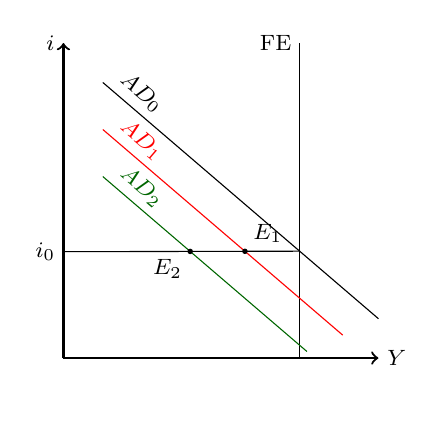
\begin{tikzpicture}
%First Graph
\coordinate (zero) at (0,0);
\draw[thick, ->] (zero) -- (4,0) node[right]{$Y$};
\draw[thick, ->] (zero) --  (0,4) node[left]{$i$};



\draw[name path = FE] (3,0) -- (3,4) node[left]{FE};

\draw[name path = AD0] (0.5,3.5) -- node [pos = 0.1, sloped, above] {$AD_0$} (4,0.5);
\draw[name path = AD1, yshift= -2em, shorten >= 2em, red] (0.5,3.5) -- node [pos = 0.1, sloped, above] {$AD_1$} (4,0.5);
\draw[name path = AD2, yshift= -4em, shorten >= 4em, black!60!green] (0.5,3.5) -- node [pos = 0.1, sloped, above] {$AD_2$} (4,0.5);



\coordinate[name intersections={of=AD0 and FE,by=E0}];
\node[left] at (0,1.35)(i0){$i_0$};

\draw[name path= i0] (E0) -- (i0);

\coordinate[name intersections={of=AD1 and i0,by=E1}];
\coordinate[name intersections={of=AD2 and i0,by=E2}];

\node[above right] at (E1){\footnotesize $E_1$};
\fill[black] (E1) circle (1pt);

\node[below left] at (E2){\footnotesize $E_2$};
\fill[black] (E2) circle (1pt);
\end{tikzpicture}
  \caption{A subfigure}
  \label{fig:sub1}
\end{subfigure}%
\begin{subfigure}{.5\textwidth}
  \centering
  \begin{tikzpicture}[decoration={triangles}]

%second Graph
\coordinate (zero) at (0,0);
\draw[thick, ->] (zero) -- (4,0) node[right]{$Y$};
\draw[thick, ->] (zero) --  (0,4) node[left]{$TB$};
\draw[thick, ->] (zero) --  (0,-2);


\draw (3,-2) -- (3,4) node[left]{FE};
\coordinate (e0) at (3,0);
\coordinate (e1) at (2.5,-0.6);
\coordinate (e2) at (2.25, 0);
\coordinate (e1p) at (2,-1.15);
\coordinate (e2p) at (0.5,0);




\node[below right]  at (e0) {$E_0$};
\node[below right] at (e1) {$E_1$};
\node[above] at (e2) {$E_2$};
\node[below] at (e1p) {$E_1'$};
\node[above right] at (e2p) {$E_2'$};



\draw[postaction={draw,decorate}, red](e0) -- (e1);
\draw[postaction={draw,decorate}, red](e1) -- (e2);

\draw[postaction={draw,decorate}, black!60!green](e1) -- (e1p);
\draw[postaction={draw,decorate}, black!60!green] (e1p) -- (e2p);


\fill[black] (e0) circle (1pt);
\fill[red] (e1) circle (1pt);
\fill[red] (e2) circle (1pt);
\fill[black!60!green] (e1p) circle (1pt);
\fill[black!60!green] (e2p) circle (1pt);


\end{tikzpicture}

  \caption{A subfigure}
  \label{fig:sub2}
\end{subfigure}
\caption{Graphs showing effects of external negative shocks in fixed exchange rate regimes}
\label{fig:test}
\end{figure}



%Back to TB=0 and FE after roughly 3 years

Start from FE and $TB=BB+PB=\emptyset$

$$\downarrow X^d, \uparrow M^d \implies$$
$$ \implies \downarrow AD \implies \downarrow Y \implies \downarrow TaxRev \implies BD$$
$$\downarrow Y \implies \uparrow U \implies \uparrow Tr \implies BD$$

$$\downarrow X^d, \uparrow M^d \implies$$
Trade deficit $\implies \uparrow$ External debt, or $\downarrow$ CB's \$ Reserves $\implies$ Because this is unsustainable for a long time, inv/spec start believing that the gov will soon eliminate the deficit, in one of two ways: 

\subsubsection{Austerity}

If it wants to remain in fixed rates:
$$ \left\{\begin{array}{l}
         \downarrow G^d  \\
          \uparrow t, \downarrow Tr \implies \downarrow Y_{disp} \implies \downarrow C^d
    \end{array} \right\} \implies$$ 
    
    $$ \implies \downarrow DD \implies \left\{\begin{array}{l}
          \downarrow AD \implies \downarrow Y \implies \uparrow U \\
          \downarrow M \implies \downarrow TD \text{ to } \emptyset
    \end{array} \right\}E_1 \rightarrow E_2 $$

\subsubsection{Let the currency depreciate}
$$1R=1P \rightarrow 2P$$
$$1P=1R \rightarrow 0.5R$$

$$\left\{ \begin{array}{l}
     \uparrow (P_M)_P \implies \text{ after 1 year a significant } \downarrow M^d \\
\downarrow (P_X)_P \implies \text{ after 1 year a significant } \uparrow X^d
\end{array} \right\} \implies$$


$$ \implies \left\{\begin{array}{l}
     \uparrow AD\text{ ... FE after 3 years } E_1\rightarrow E_2  \\
     \downarrow TD \text{ ... } TB=\emptyset 
\end{array} \right\} $$

Conclusion: $\downarrow NX^d \implies$ benefit of a depreciation on the medium term. 

A return to $TP=\emptyset$ with $\downarrow U$ instead of a return to $TP=\emptyset$ with a further $\uparrow U$ (as would happen with austerity).

\subsubsection{Costs of letting a currency depreciate}

The benefit of leaving fixed rates are bigger when the size of the external shock is bigger. 

A depreciation implies severe costs in the short run:
\paragraph{1.}
Imported goods becomes more expensive, CPI rises, pruchasing power of the population goes down. Initiates a spiral, where, workers demand higher nominal wages, unit costs increase and prices of domestically produced goods rise as well. 

$$\uparrow (P_M)_P \implies \uparrow CPI \implies \downarrow \text{ Purchasing power} \implies \text{spiral:} \uparrow W_N \implies \uparrow UC \implies \uparrow \text{Price of domestic goods} \implies$$
$$\implies \uparrow \pi$$

Increase in expenditure on imported goods, less income to spend on domestic goods, Decline in AD, decline in Y, and increase in unempoyment. 

\paragraph{2.} 

Domestic firms and banks partly fund themselves in many countries, through foreign loans in \$. That they then exchange for pesos with the central bank (the interest rate on \$ loans is normally lower). 

As a result: The currency depreciates, the value of debts go up. Value of those debts. Consequence: Firms profits decline, Investment demand declines, AD goes down, income goes down. Unemployment goes up. 

Unemployment in the short term is likely to rise following a depreciation.

$$dep \implies losses \implies \downarrow EqK \text{ below 10\% loans} \implies \text{banks are forced to reduce loans} \implies$$
$$\implies \downarrow (C^d+I^d) \implies \downarrow AD \implies \downarrow Y \implies \uparrow U$$

\section{Review of second generation models}

Starting from full EQ: (E0)
Full employment and TB = 0

External negative shock: 


$$\begin{array}{lcl}
\downarrow X^d & \implies & \downarrow AD \implies \downarrow Y \implies \uparrow U \\
\uparrow M^d & \implies & \uparrow D \implies \uparrow \text{External Debt and/or CB \$ reserves} \\
\end{array}$$

Speculators and IFI start to belive that the government will eliminate the TD in one of 2 ways:

1. Austerity: 
$$\downarrow G^d, \underbrace{\downarrow TR, \uparrow t}_{ \downarrow C^d} \implies \downarrow DD \quad  \begin{array}{|lll} \implies \downarrow AD \implies \downarrow Y \implies \uparrow U \\ \implies \downarrow M \implies \downarrow TD = \emptyset \end{array}$$


Decline in external demand worsens TB, incre .... 

2nd option: Leave fixed rates and let the currency depreciate, after 1 year 

$$\begin{array}{l|ll}\uparrow X^d & \implies & \uparrow AD, \uparrow Y, \downarrow U \\ \downarrow M^d & \implies & \downarrow TD\end{array} \ldots \text{FE}$$

after 3 years back to FE

ii is better than i, why? It allows a return to a TB eq, with a reduction in unemployment instead of a TB = 0 with increased unemployment. 

%COST BENEFIT GRAPH

However, a depreciation implies costs in the short term:
Reasons:
$$\uparrow (P_m)_p \quad \begin{array}{|ll}\implies \uparrow \text{CPI} \implies \downarrow PP \implies \text{Spiral} \implies \uparrow W_N \implies \uparrow \text{UPC} \implies \uparrow P \text{ domestic goods} \implies \uparrow \pi \\ \implies \uparrow \text{Expenditure on imported goods} \implies \text{Less income for domestic goods} \implies \downarrow AD, \downarrow Y, \uparrow U \end{array}$$
The price of Argentinian import goods increase, the CPI increases and thus purchasing power decreases. It leads to a spiral where workers demand higher nominal wages, which leads to production costs increases, which increases \textbf{Domestic} prices. 


When people pay more for imported goods, less money left for domestic consumption. Thus, domestic firms face less demand, they produce left and will have to fire some workers. 

Another reason why a deprecation tends to increase U in the short term:

Domestic banks and firms are typically indebted in dollars towards foreign banks. 
Result:
Depreciation increases the value of the foreign debt denominated in Pesos. This also increases the value of interest payments on the foreign loans. 

Thus, firms profits fall because their debt is more expensive, their investment drops, leads to lower demand and output and higher U. 

The most important reason for U increase after depreciation:
The equity of banks, the value of their assets minus their liabilities. Their assets are domestic loans in local currency, debts, partly in dollar. Because of the depreciation their equity drops because their liabilities increase. If it falls below 10 \%, they have to reduce their extension credits to household and businesses, as they are required by law to keep 10 \% of their liabilities. As a result, demand, and output go down which increases unemployment. 

Three sorts of costs:
\begin{enumerate}
    \item Consumers can buy less
    \item Higher inflation
    \item Higher unemployment
\end{enumerate}


A bigger negative external shocks has higher costs in the short run. 

\subsection{First reason of a flight of the local currency (Krugman, II)}

The two actors who flee the domestic currency are International investors and speculators because of a negative external shock. 

Investors and speculators believe that the shock is of a larger type, $\downarrow NX^d$, and increasing the benefit of a depreciation above the costs even though the Gov is still hesitant whether to depreciate or not. 

They flee out the currency, a sharp decline in dollar reserves of the central bank. Facing this sharp decline in dollar reserves, knowing that the medium term benefit of the depreciation will outweigh the short term costs, they are no longer hesitant to depreciate the currency. 

Speculators will profit of the depreciation by short-selling the currency, they have an incentive to flee when suspecting that they currency will depreciate. 

What if the predicted depreciation does not materialise?

Speculators will have to pay back what they borrowed + interests, which can be high as a deterrent for this speculation. Only a small loss, 2\% of the borrowed amount if interest rate is 100\% p.a. 

Speculation in fixed rates is a one-way bet because the possible gain is much higher than the loss. 

\subsection{2nd reason for a flight (Obstfeldt, 1986)}
Investors and speculators believe that the shock has been small. The shock has increased the benefits of a depreciation, but still at a level that is lower than the costs. Thus, the government has little interest to depreciate, because the costs are higher than the benefits. However, speculators know that they have the power to increase further the benefits of a depreciation above its costs. How?

If they carry massive short-sales of the currency, the CB will have to defend the value of the currency. Not only by selling its dollar reserves, but also raising interest rates to very high levels.

This rise increases the returns of the IFI, if they stop fleeing out of the currency and stick their SD in P. In addition it is more expensive to short sell.

\textbf{Key point:}
The interest rate is very high, decline in AD, to i3 in graph. Output down, U up, Move from E2 to E3 in graph. 
The benefit of depreciation increase, the government has incentive to let the currency depreciate (Bank of England 1992), speculators make huge profits. 

\subsection{Adjustment problem}

   $$\downarrow NX^d \implies \uparrow \text{benefits of depreciation relative to costs} \implies \text{IFI + Spec} \implies \text{flee short} \implies  $$
   $$\implies \text{forcing the country to leave fixed rates}$$


Benefits of depreciation: increases competitivness

\subsection{The $n - 1$ problem}

	Under fixed rates and perfect financial capital mobility.
	
	$$\text{(FRP)} = 5\%$$
	
	$$i_1 = i_2 = \ldots = i_N$$
	
	If $$i_1 < i_2 = \ldots = i_N$$
	The speculators and investors will flee, leading to a quick deplation of the CB’s dollar reserve.

The country has 2 choices:
\begin{itemize}
    \item 	Raise the interest rate back to the intial level
    \item	With no remaining reserves, they will have to move to a floating rate system 
\end{itemize}


In the EMS 1979-1989 nearly all EMS countries registered double digit inflation - with a big exception, Germany.

The other countries wanted to lower their inflation, they formed a strategy known as the exchange rate anchor, which involved pegging the currency to the Deutsch Mark rate. Guaranteed a reduction in  inflation to Germany level. To make this possible they had to follow Germanys interest rate.

After the reunificiation of germany in june 1990, government had to lend huge sums with the integration of East Germany, which pushed inflation in Germany up, forcing the CB to rise interest rates, and forcing other countries of the EMS to rise their interest rates. 

$$\text{AD} \uparrow \implies \downarrow U \implies \uparrow \pi_G \text{from 0\% (1998 to 6\%(1992)} \implies \uparrow i^G_{CB} \text{from 4\% in 1995 to 10\% in 1992}$$

Because of fixed rates, and perfect capital mobility, the BOE was forced to $\uparrow i_{UK}$ from 4\% in 19987 to 15\% in sep 1992. Risk premium on british bills.

The high interest rate led to a decline in the willignes to extend credit for consumption and investment. A decline in DD with 2 effects. Imports fall, the trade balance improves. In the case of Britian the trade deficit went from -3.5\% of GDP in 1990 to -1\% in 1992. 

The adverse effect is a decline in output and an increase in unemployment from 7\% in 1990 up to 11\% in december 1992. A rapid increase in U. Loss of purchasing power in the case of depr.

A possible increase in inflation because they might demand higher nominal wages, cost of production rise, they raise their prices. 

An important cost in the british case. Uncertain exchange rates with other currencies, it imposes a cost on international trade and to foreign direct investment in UK. 


In the first half of 1992, the british gov said repeatedly it would not leave EMS, and let the £ depreciate (presumably because costs>benefits). 

However, Soros didn't only bet on the depreciation of the £, he engineered it (Obstfeld, 1986). 

\subsubsection{Consequences for the British Economy}

\begin{enumerate}
    \item The £ then stabilised at a value 15\% below it's initial value $\uparrow X, \downarrow M \implies \uparrow AD$
    \item Floating rates then allowed the BOE to $\downarrow i$ to 6\% in '94 $\implies \uparrow \text{credit}$ to $(C^d+I^d) \implies \uparrow AD \implies \uparrow Y \implies \downarrow U$ from 11\% in Dec'92 to 6\% in '99 vs $U\simeq 10\%$ in France and Germany.
\end{enumerate}

\subsection{The end of the Bretton Woods system of fixed rates between USD, DM, franc, Yen}
 A system that existed between 1949 and 1973, the root cause of the collapse was the implementation of the very expansionary fiscal policy after 1966:
 \begin{itemize}
     \item Increased military spending caused by the intensificiation of the Vietnam War
     \item The great Society program, increase in public expenditure in social areas. Education, health (medicare: paying all medical expenses of the elderly, with the exception of prescription drugs) To combat poverty
     \item Succesful, reduced population below poverty line from 22,5 to 12,5 in 10 years. 
 \end{itemize}

$\uparrow G_{Annual}^{Nominal}$ from 5\% in the years up to 1965, up to 11\%-15\% in 1966-1969. 

 - Increase in the emission of treasury bonds, bought by banks. Increase in $g_{CD = MS} \implies \uparrow g_{MB}$

$$\uparrow DD \implies$$

$$\uparrow M \implies TB < 0$$

The TB went from a surplus of 6 billion usd (1965) to zero in (1969) and to a deficit of 5 billion by 1972. (The bad side)

$$\uparrow AD \implies Y \implies \downarrow U \implies  \uparrow g_{W_N} \implies \uparrow g_{UC} \implies \uparrow g_{P} \implies \uparrow \Pi$$
Unemployment went from 5\% in 1962-5 to 3.5\% in 1966-69. The workers increased their bargaining power. As a result inflation grew from 1.5\% in 1964 to 6\% in 1970. 

Consequence of raising interest rate on $g_{MS}$??

Money illusion

$$g_{MS}^{annual} = 7\% - 10\%$$

$$g_{G^d}^{annual} = 11\% - 15\%$$

$$\uparrow i \implies \underbrace{g_{C^d, I^d} < g_G}_{g_{MS}}$$

Private consumption grew at a slower rate than public expenditure, possibly because of the increase in the nominal interest rate.

Quick recap:
The US fiscal expansion in the last years of the 60s, led to an increase in output, a reduction in unemployment and an increase in inflation. ON the other hand, reduced thet rade surplus which eventually became a deficit.  

\subsubsection{The effect on the European economy}
$$\uparrow DD_{US} \implies$$
$$\uparrow AD_{US} \implies \downarrow U_{US} \implies \uparrow \pi_{US}$$

The increased inflation was incorporated in  the price of US goods imported to Europe. 

$$\uparrow M_{US} \implies \uparrow X^d_{EU} \implies \uparrow AD_{EU} \implies \uparrow Y_{EU} \implies \downarrow U_{EU} < U_N \implies \uparrow g_{W_N} \implies \uparrow g_{UC_{EU}} \implies \uparrow \pi$$

Consequences if there floating rates between usd, dm, ff, etc

$$\uparrow DD_{US}\begin{array}{l}\implies \uparrow AD_{US} \implies \downarrow U_{US} \implies \uparrow \Pi_{US} \\ \implies \uparrow M_{US} \implies \uparrow X_{G} \uparrow \implies AD_{G} > FE\end{array}$$

$$\uparrow \pi_{EUR} \text{ from 3\%(1966) to 6\%(1972)}$$
$$\uparrow \pi_{G} \text{from 2\%(67-69) to 6\%(1972)}$$
. 

The increase in exports in Europe led to a trade surplus, especially in Germany. 

$$\left\{\begin{array}{l}
     \uparrow \text{ \$ Reserves of GCB} \\
     \uparrow R_{DM} \text{ in the German banking system}
\end{array} \right\} \implies$$

$$ \implies \text{ ESR in the IBMM} \implies \text{ tendency for} \downarrow i_{IBMM} \text{ avoided by the CB of Germany through sale of TB's - sterilisation}$$

tendence of decline for $\downarrow i_{IBMM}$ avoided by the CB by selling treasury bonds


\subsubsection{Consequences if there were floating rates between \$, DM, FF, etc.}

$$\uparrow DD_{US} \implies AD_{US} \implies \downarrow U_{US} \implies \uparrow \pi_{US}$$
$$\implies \uparrow M_{US} \implies \uparrow X_G \implies AD_G \text{ above FE}$$.

In floating rates the surplus in dollars isn't exhanged by the CB, and the DM would appreciate. 

\paragraph{Consequences for the apreciation of the DM}

\begin{itemize}
    \item $\uparrow \pi_{US}$ from 1\% to 6\% $\implies \uparrow \pi$ in the goods imported by Germany: \begin{description}
        \item $(P_M)_{\$}\text{ } 1\$ \longrightarrow 1.06\$$
        \item $(P_M)_G\text{ } 1DM \longrightarrow 1DM$
    \end{description}
    \item $\uparrow(P_X)_G^{\$} \implies \downarrow X^d_G \implies \downarrow AD_G$ towards FS $\implies no \uparrow (g_{w_N})_G$
\end{itemize}

In sum, $\uparrow DD_{US} \implies \uparrow \pi_G$ if fixed rates, and $\uparrow DD_{US} \centernot\implies \uparrow \pi_G$ if floating rates. 

Understanding that Germany would want to stop the $\uparrow \pi$ and therefore would want to leave fixed rates and let the DM appreciate, 

$$IFI/spec \underset{\rightarrow}{DM} CG_G\implies \uparrow \text{\$ Reserves of the } CB_G=215\%$$

Which ultimately ended the Bretton Woods system.


\end{document}
